\documentclass[11pt]{article}

% package to include images
\usepackage{graphicx}

% parameters for \maketitle
\title{Computational Vision Lab 01}
\author{Johannes Heidecke}

% paragraph formatting
\setlength{\parindent}{2em}
\setlength{\parskip}{2em}
\renewcommand{\baselinestretch}{1.1}

% prevent orphans and widows
\widowpenalty10000
\clubpenalty10000

\begin{document}

\maketitle


\section*{Exercise 1:}

The three gray scale images are created in Matlab as simple matrices containing zeros and ones. These matrices are then concatenated along the third dimension to form the three color channels of the RGB image. See figure \ref{fig:task1}.

\begin{figure}[!hbt]
  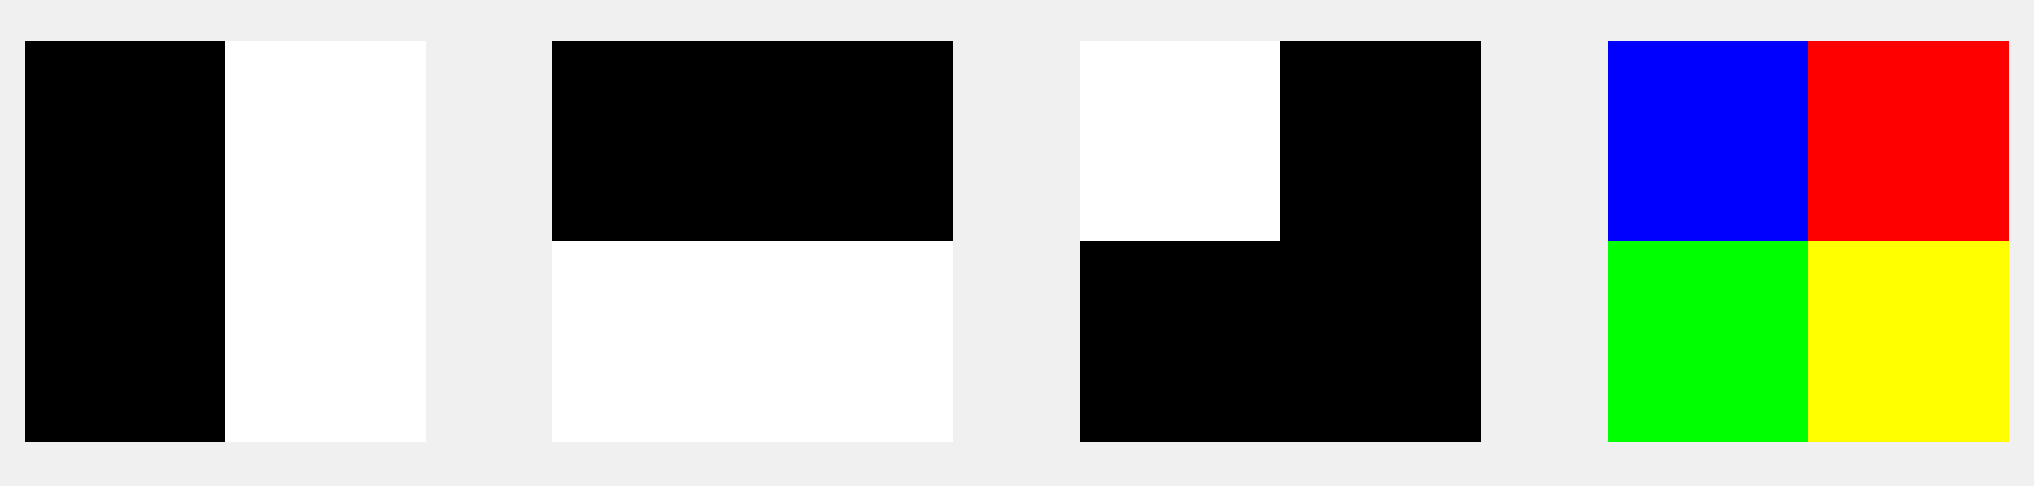
\includegraphics[width=\textwidth]{task1}
  \caption{Results of Exercise 1}
  \label{fig:task1}
\end{figure}


\section*{Exercise 2:}

The image \textit{chairs.jpg} consists of the three different color channels of the RGB spectrum: red, green and blue. Pixel that have a high portion of red color (e.g. the pillows on the chairs) have a very high value in the red color channel. Looking at the greyscale image of this channel, these pixels appear almost white. The very red pillows appear black in the green and blue channel, since their color does not contain a lot of green and blue. Colors that have a almost equal distribution of the three channels are perceived as the range from white, to gray, to black. The image contains mainly white and gray colors, for that reason the three channels look very much alike, as can be seen in figure \ref{fig:task2}.

\begin{figure}[!hbt]
  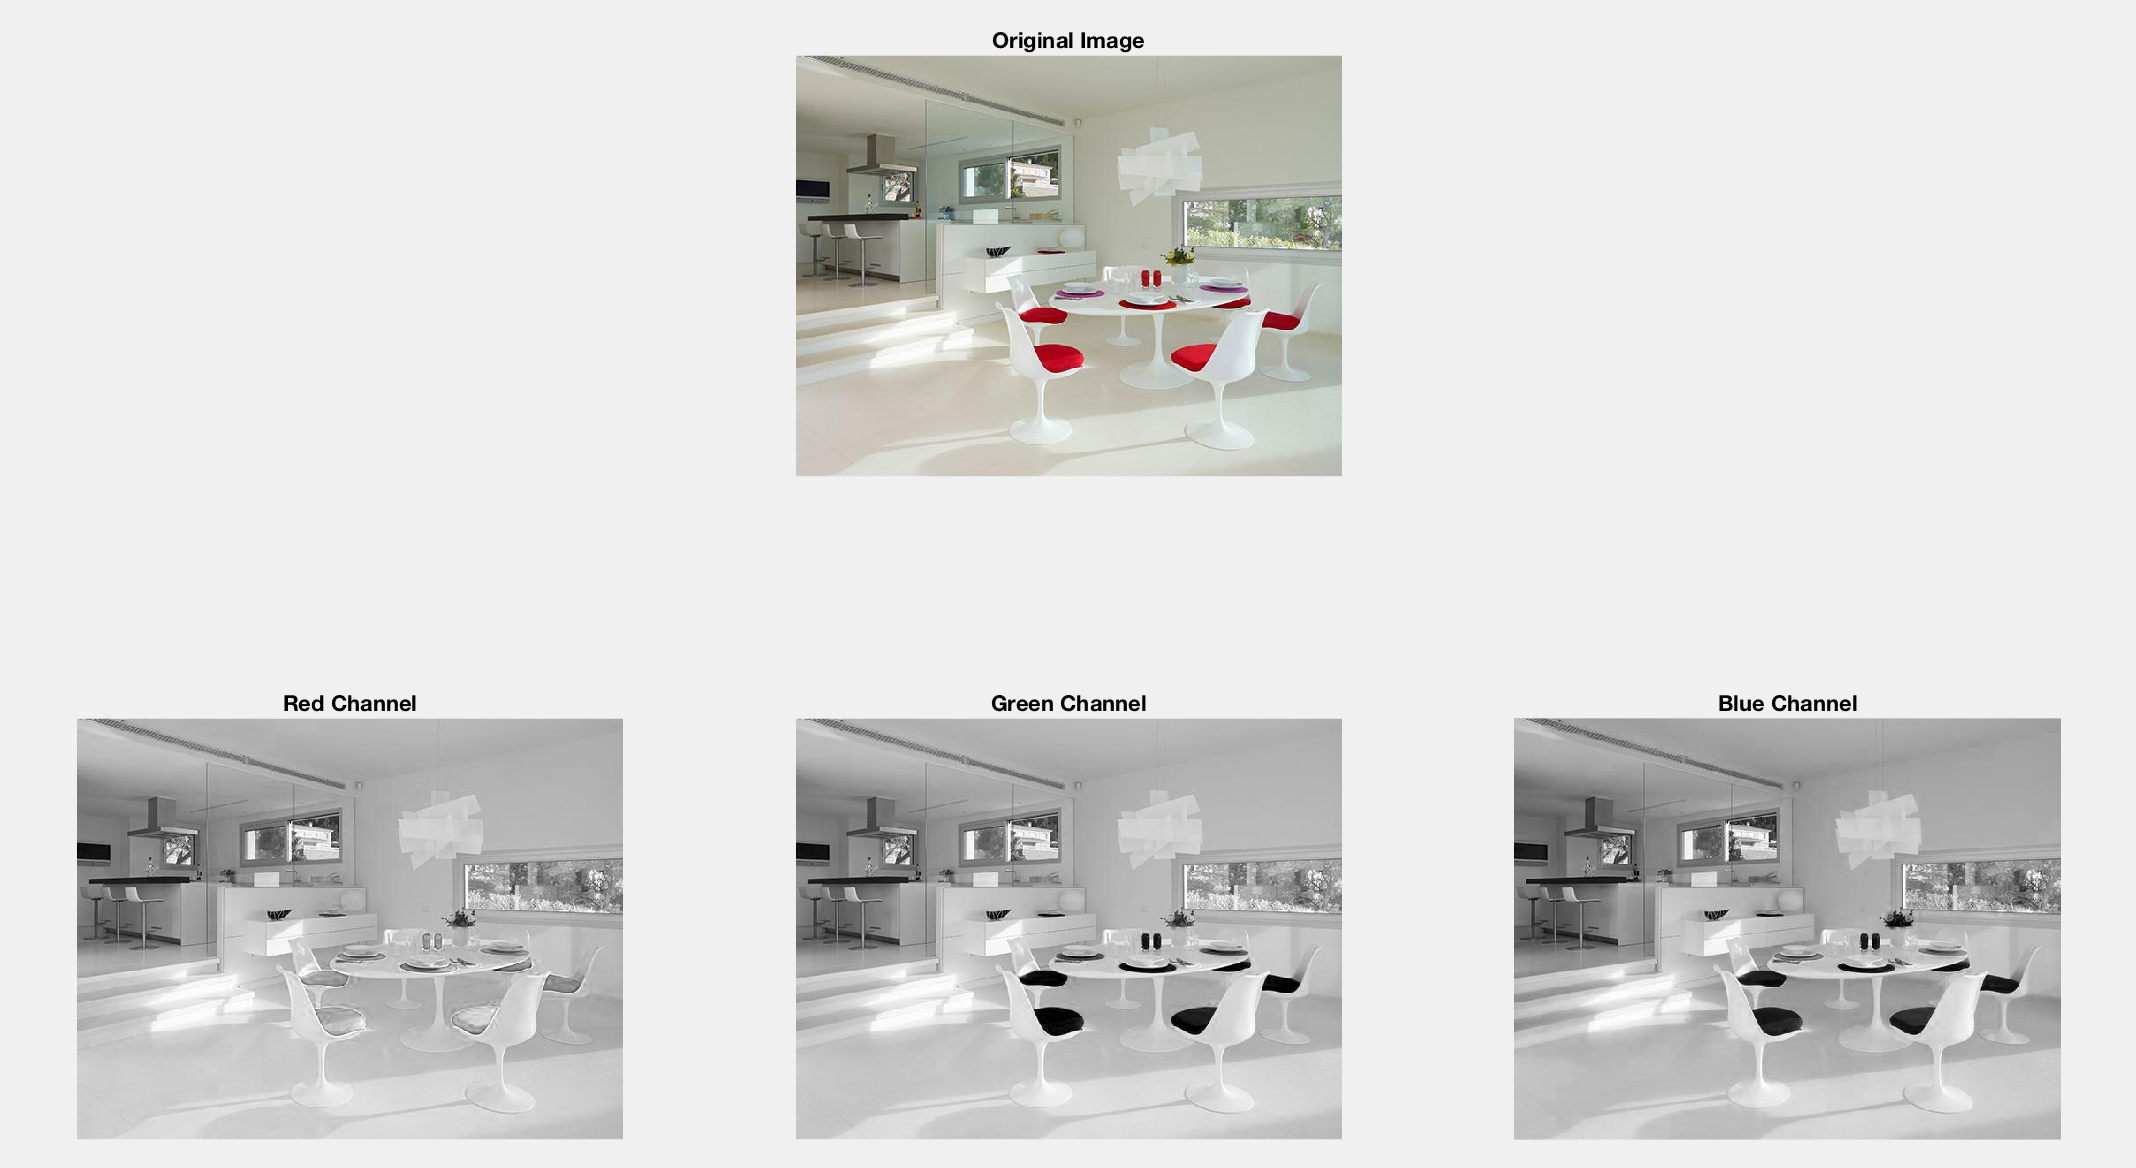
\includegraphics[width=\textwidth]{task2}
  \caption{Original Image and its three RGB channels}
  \label{fig:task2}
\end{figure}

It is possible to interchange the different channels with each other. Since there are three channels, 6 different permutations are possible, with one of them being the normal RGB order. The results of those permutations can be seen in figure \ref{fig:task3}.

\begin{figure}[!hbt]
  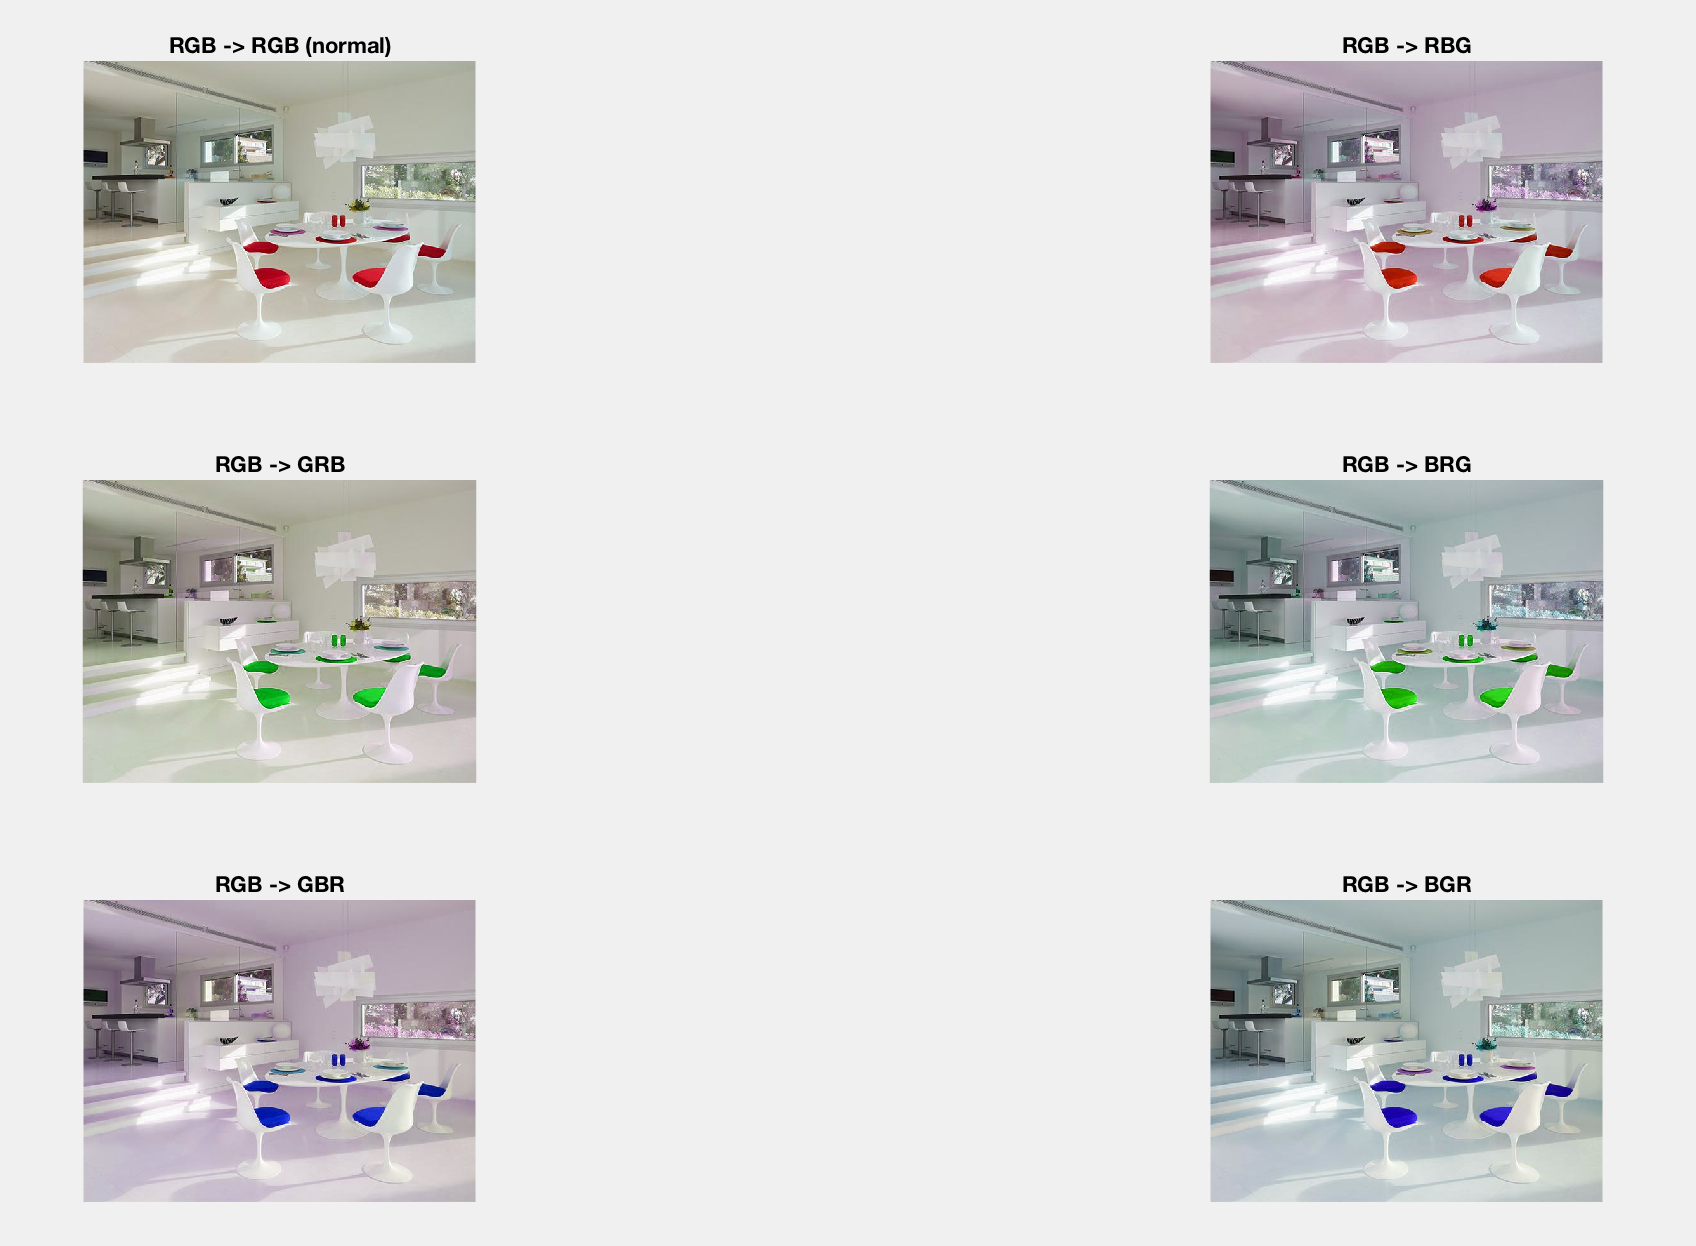
\includegraphics[width=\textwidth]{task3}
  \caption{Interchanging the RGB channels}
  \label{fig:task3}
\end{figure}

It is also possible to completely turn off single channels by multiplying all values of a channel by zero. The resulting images are colored in cyan, magenta, and yellow - exactly the colors that are being used in the subtractive color model of printing. The results are shown in figure \ref{fig:task4}.

\begin{figure}[!hbt]
  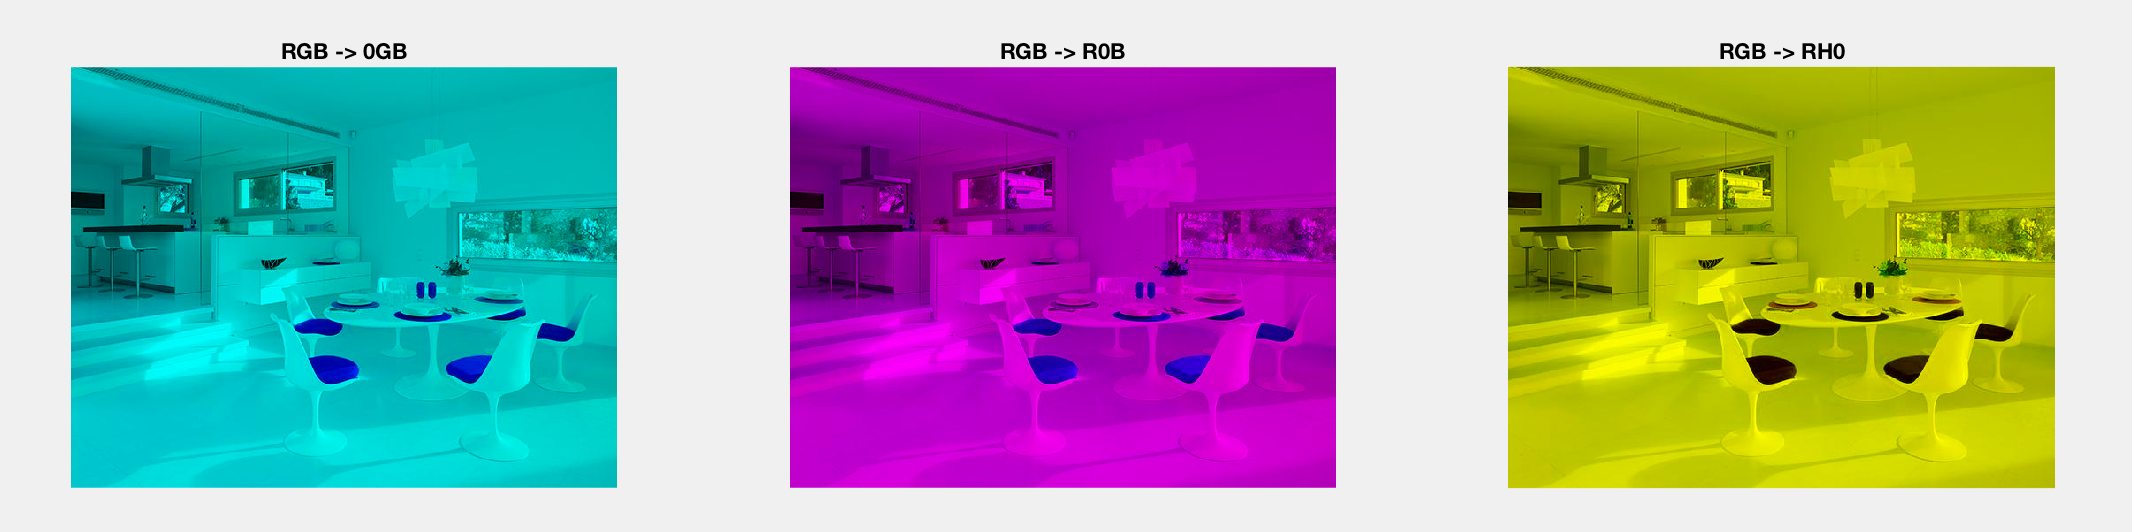
\includegraphics[width=\textwidth]{task4}
  \caption{Deactivating single RGB channels}
  \label{fig:task4}
\end{figure}

\section*{Exercise 3:}

Resizing an image to a smaller size reduces not only the size but also the details of the image. This can be seen in figure \ref{fig:task5}. While a rescaling to 0.5 times the original size still shows most of the details of this particular image, after rescaling it to 0.01 size almost all details are lost.

\begin{figure}[!hbt]
  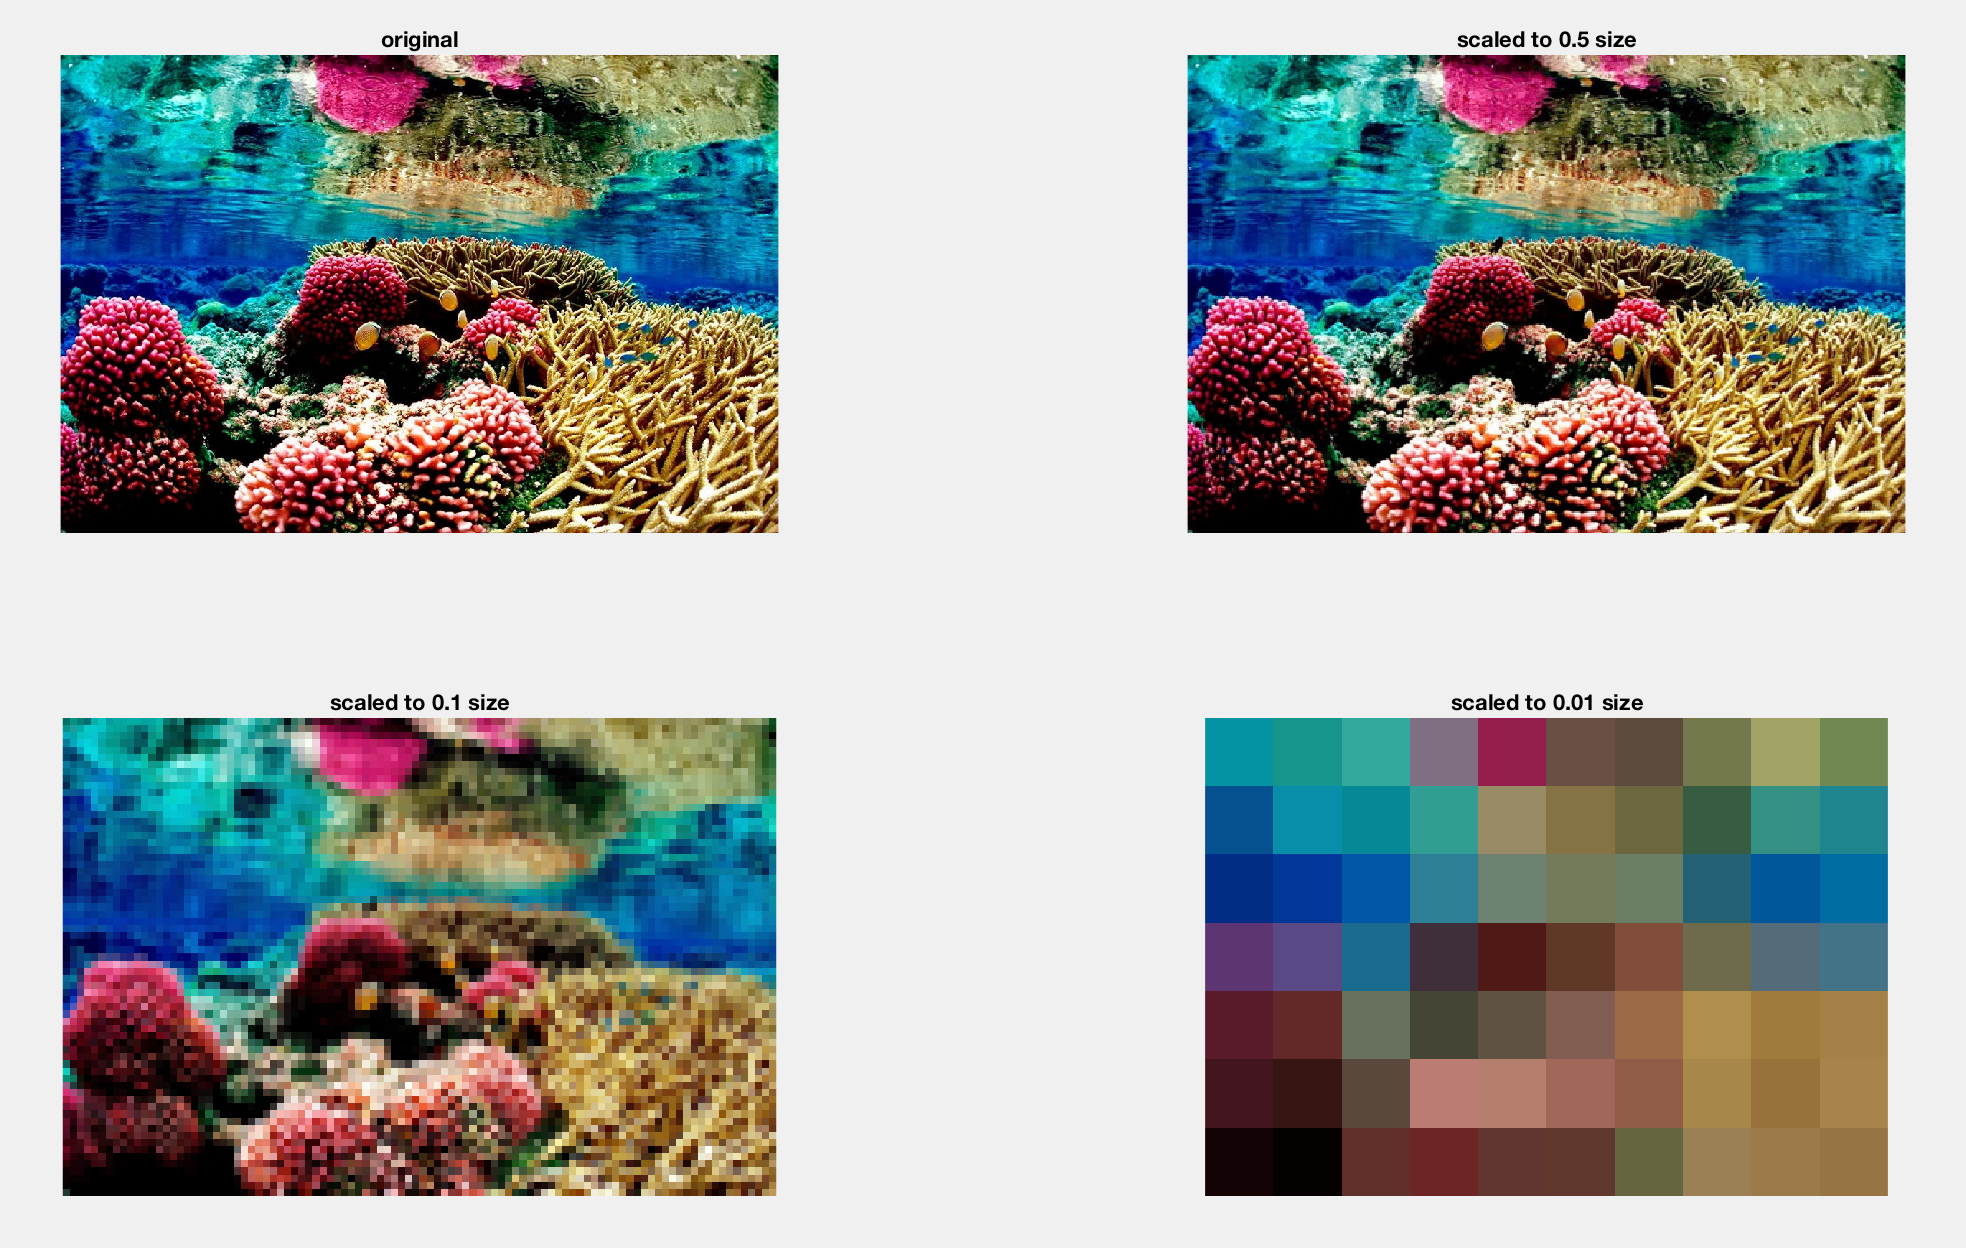
\includegraphics[width=\textwidth]{task5}
  \caption{Resizing the original image to smaller sizes}
  \label{fig:task5}
\end{figure}

This loss of details after resizing can also be observed in the histogram of the three color channels. In figure \ref{fig:task6} the three histograms of the RGB-channels of the original image are shown in the left column. The same histograms are shown on the right, after reducing the size to 10\% of the original size. It can clearly be observed that after resizing, the channels' values are less smoothly distributed and are concentrated on a smaller number of distinct values. This is an effect of combining the values of several pixels into one in order to allow a smaller size. 

\begin{figure}[!hbt]
  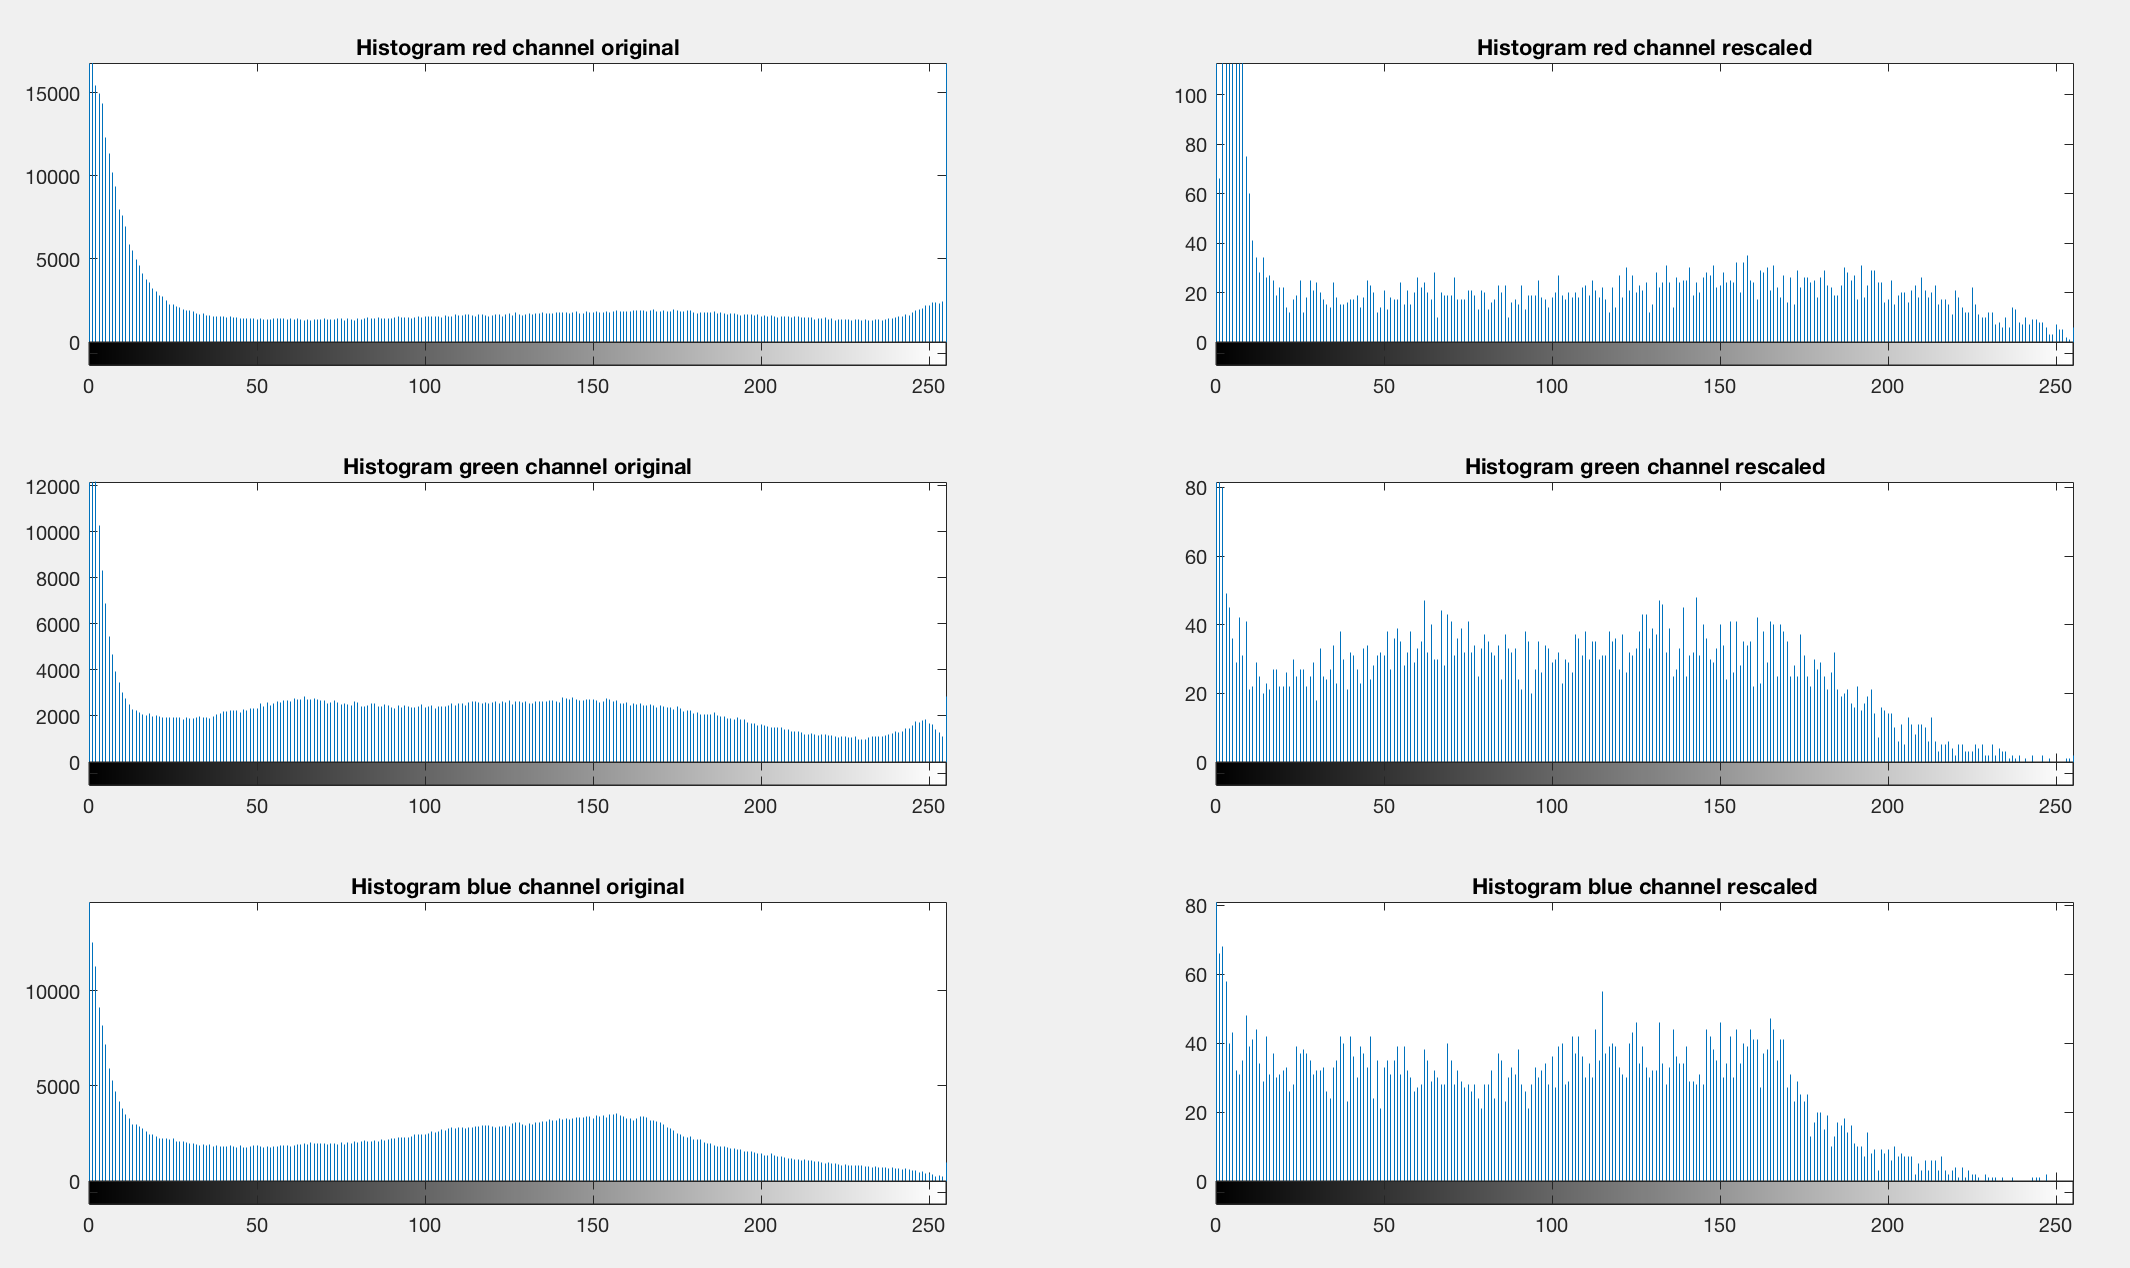
\includegraphics[width=\textwidth]{task6}
  \caption{Change of the RGB histograms after resizing to 0.1 original size}
  \label{fig:task6}
\end{figure}

It is possible to return the smaller image back to its original size. As figure \ref{fig:task7} shows, the restored image does still not show the same amount of details as the original image. The details that were lost in the small image in the middle can not be re-computed. The only improvement is, that the restored image looks less pixelated, i.e. no single pixels are visible from a certain distance.   

\begin{figure}[!hbt]
  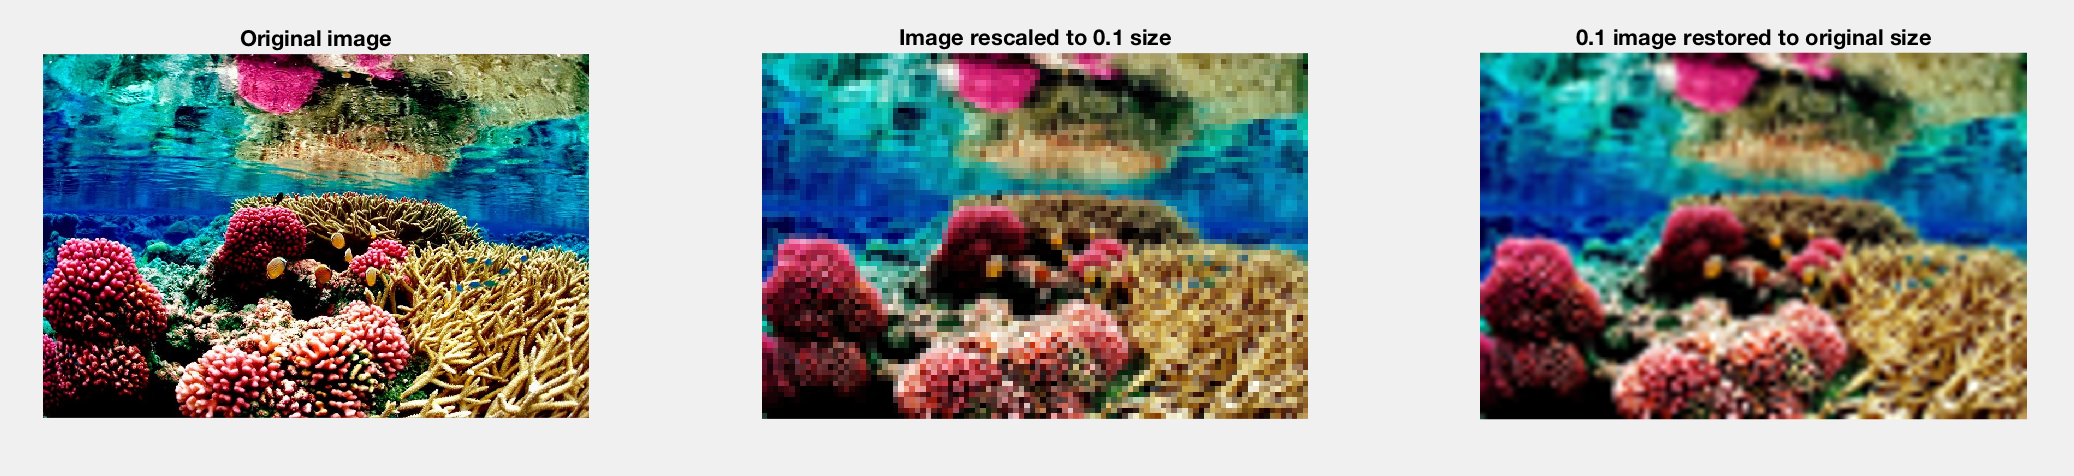
\includegraphics[width=\textwidth]{task7}
  \caption{Resizing to 0.1 size and then restoring to original size}
  \label{fig:task7}
\end{figure}

This effect can be observed better when only looking at a smaller area of the image, as in figure \ref{fig:task8}. This figure shows, that when resizing to 0.1 of original size, most details get lost and the image looks very pixelated. When restoring from the 0.1 image back to original size, the pixelated look disappears, but the former details can not be recovered.

\begin{figure}[!hbt]
  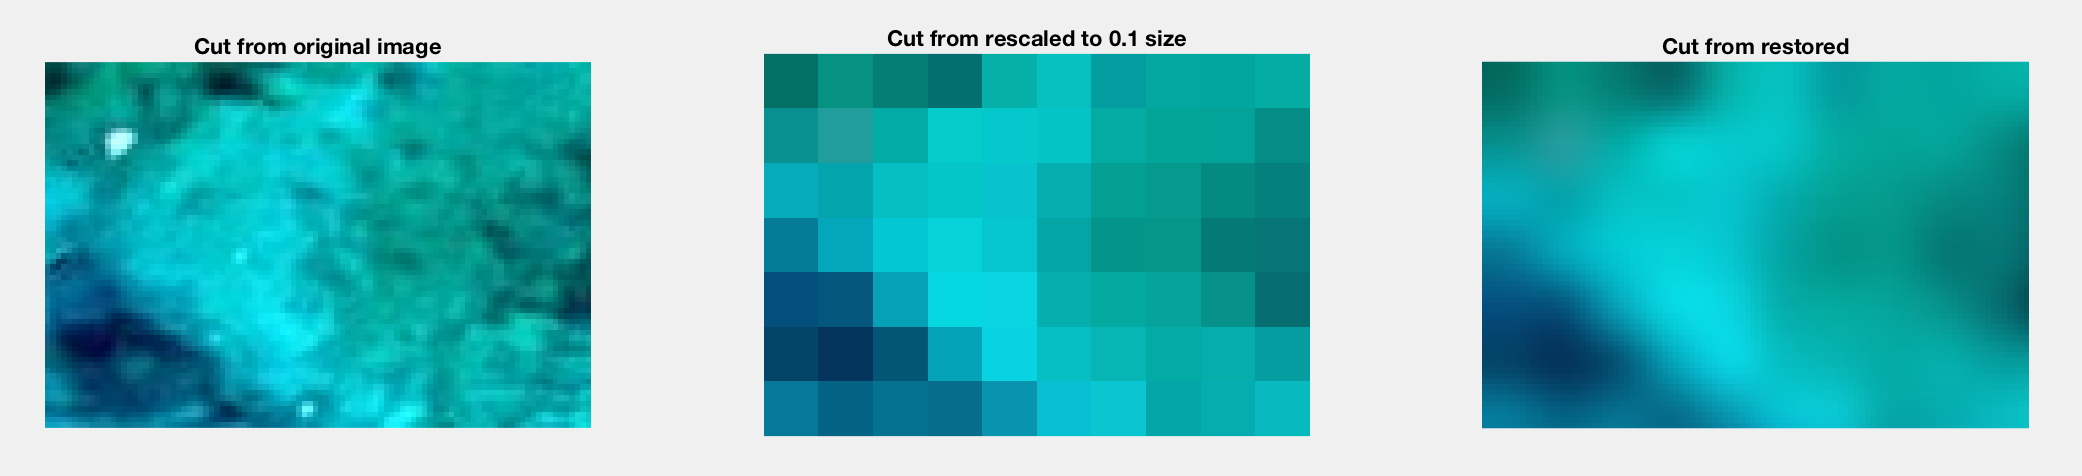
\includegraphics[width=\textwidth]{task8}
  \caption{Resizing to 0.1 size and then restoring to original size}
  \label{fig:task8}
\end{figure}

As an alternative for removing image details different smoothing filters can be applied. One option is to apply unweighted moving averages that simply add all values in the neighborhood of a pixel and then normalize the sum by dividing through the number of added pixels. In this case, the size and shape of the area that is chosen to calculate the average has a big impact on the outcome, as can be seen in figures \ref{fig:task9} and \ref{fig:task10}.

In figure \ref{fig:task9} both a horizontal filter of size 1 x 50 pixel and a vertical filter of size 50 x 1 is applied to all pixels in the image. The former results in an effect that looks like the camera was moved vertically while taking the picture, the latter like it was moved vertically. While both filters will remove some kind of noise in the image, their results still look very different. 

\begin{figure}[!hbt]
  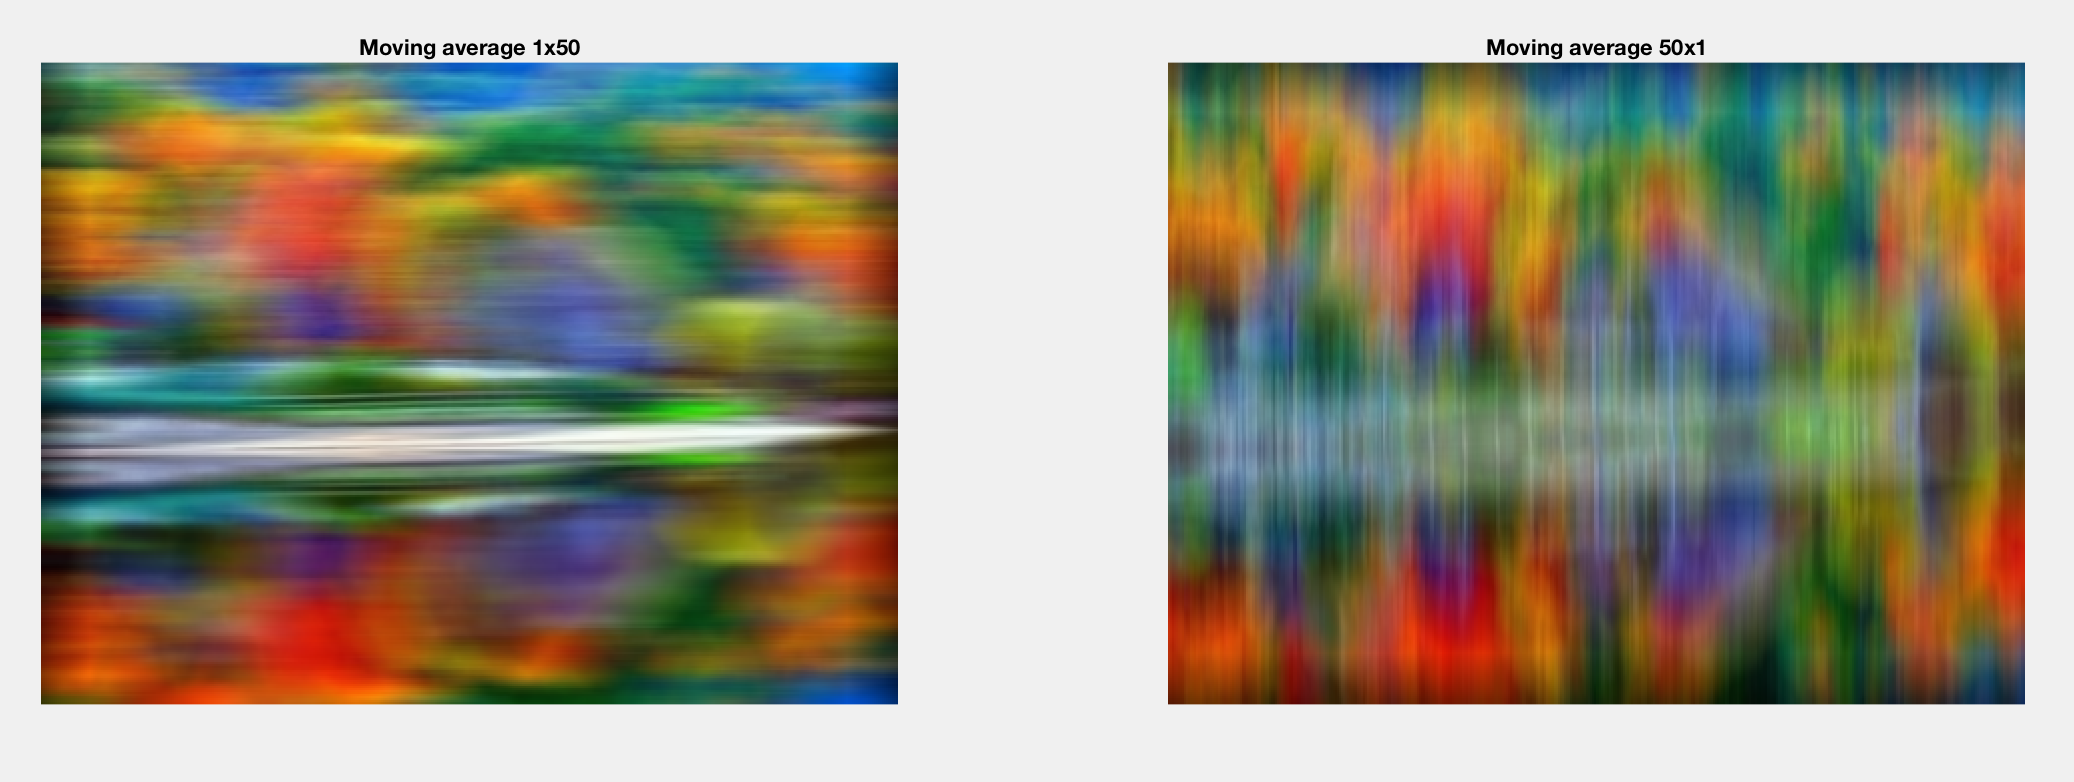
\includegraphics[width=\textwidth]{task9}
  \caption{Horizontal and vertical unweighted moving average}
  \label{fig:task9}
\end{figure}

Figure \ref{fig:task10} shows unweighted moving average filters in square shape of different sizes from 3x3 to 100x100. The filter size determines how much noise is removed but also how many details are lost. Filters with a larger area make the image more blurry and remove more details, but they also remove noise more evenly. The optimal filter sizes can vary a lot from image to image.

\begin{figure}[!hbt]
  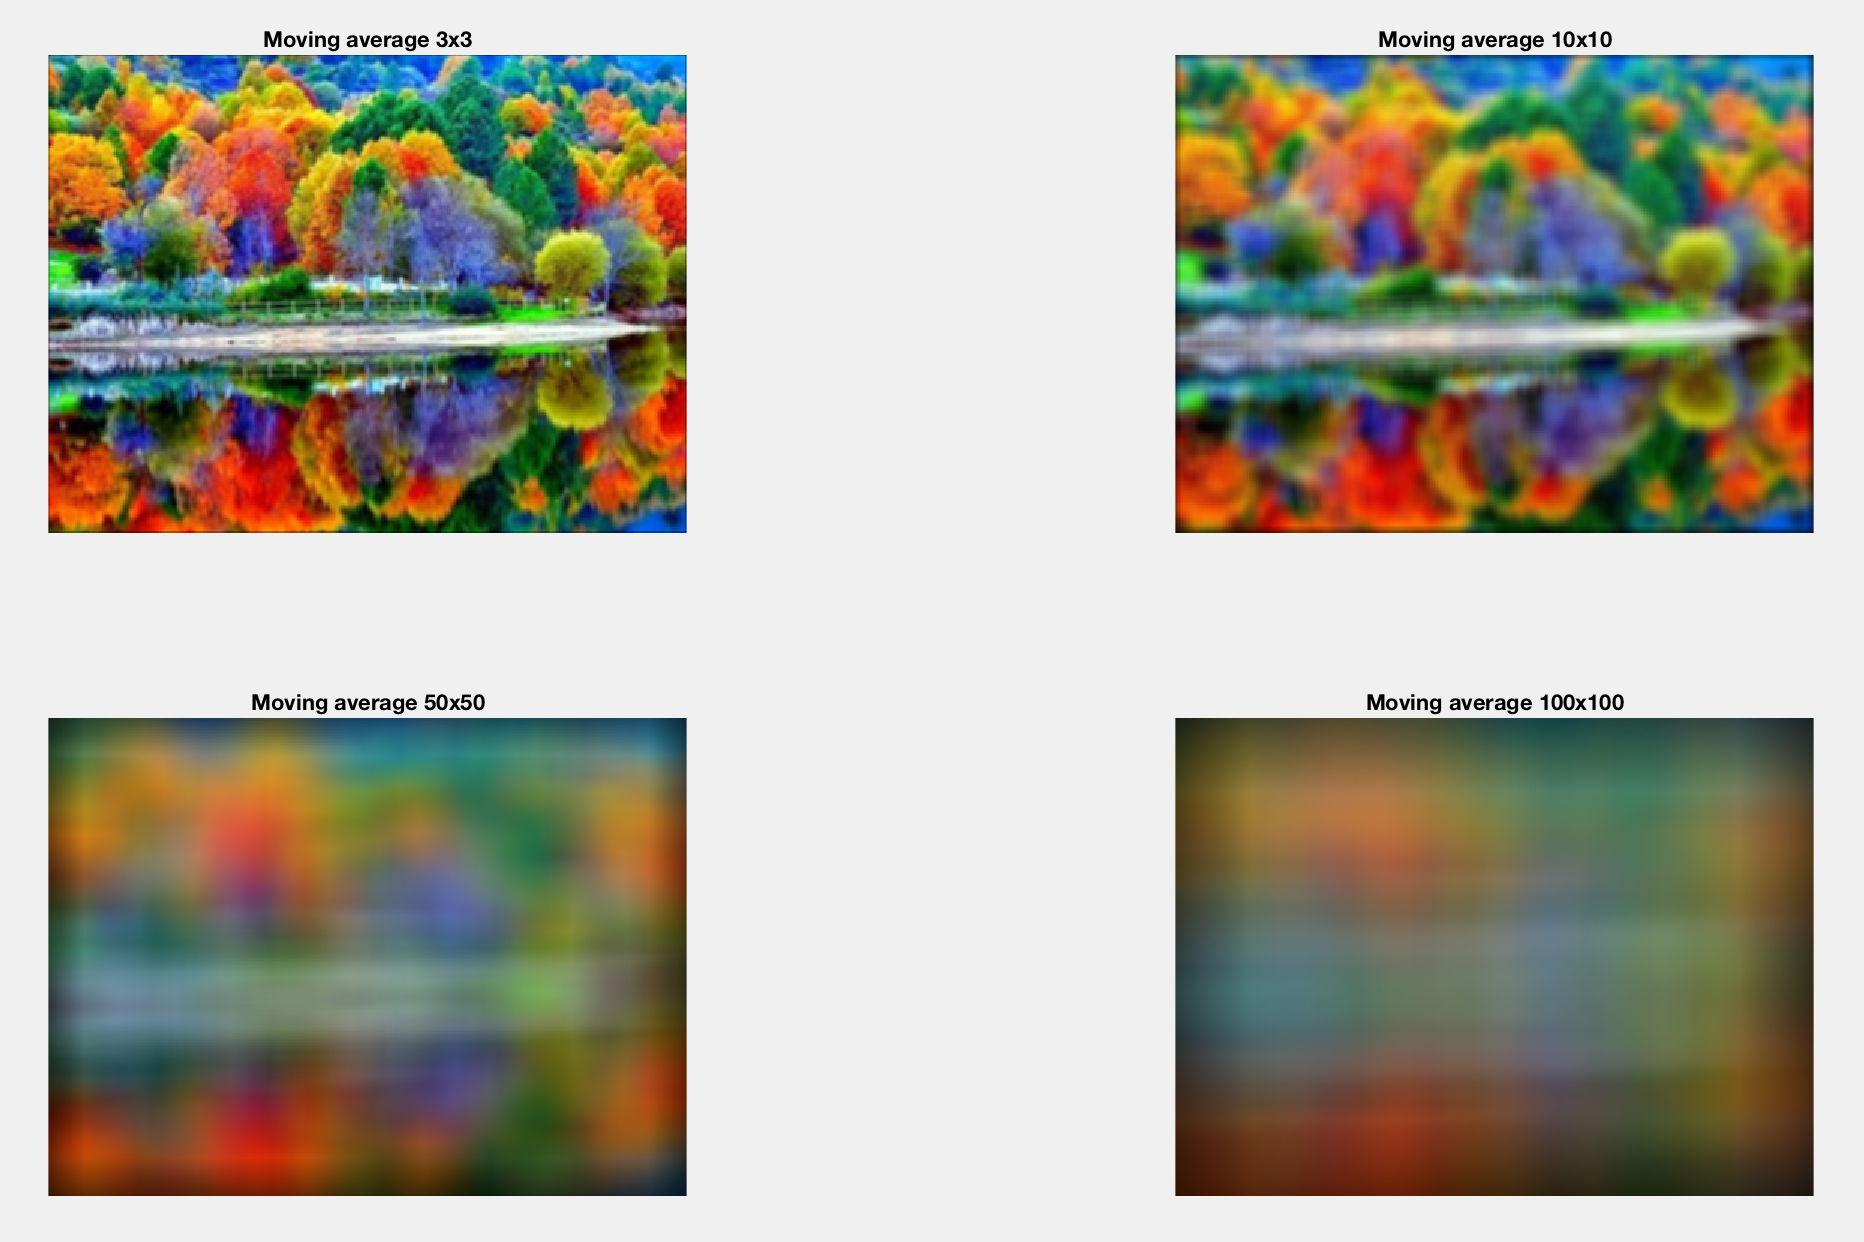
\includegraphics[width=\textwidth]{task10}
  \caption{Square shaped unweighted moving averages in different sizes}
  \label{fig:task10}
\end{figure}

Besides unweighted moving averages it is also possible to reward proximity to the target pixel by weighting close neighbors of the pixel more highly. Figure \ref{fig:task11} shows a comparison of an unweighted horizontal kernel of 1 x 10 pixel size with a weighted horizontal kernel with weights [1, 2, 4, 8, 16, 32, 16, 8, 4, 2, 1]. The unweighted filtering gives the same importance to pixels that are much further away than close neighbors and results in a more blurry picture with less details.

\begin{figure}[!hbt]
  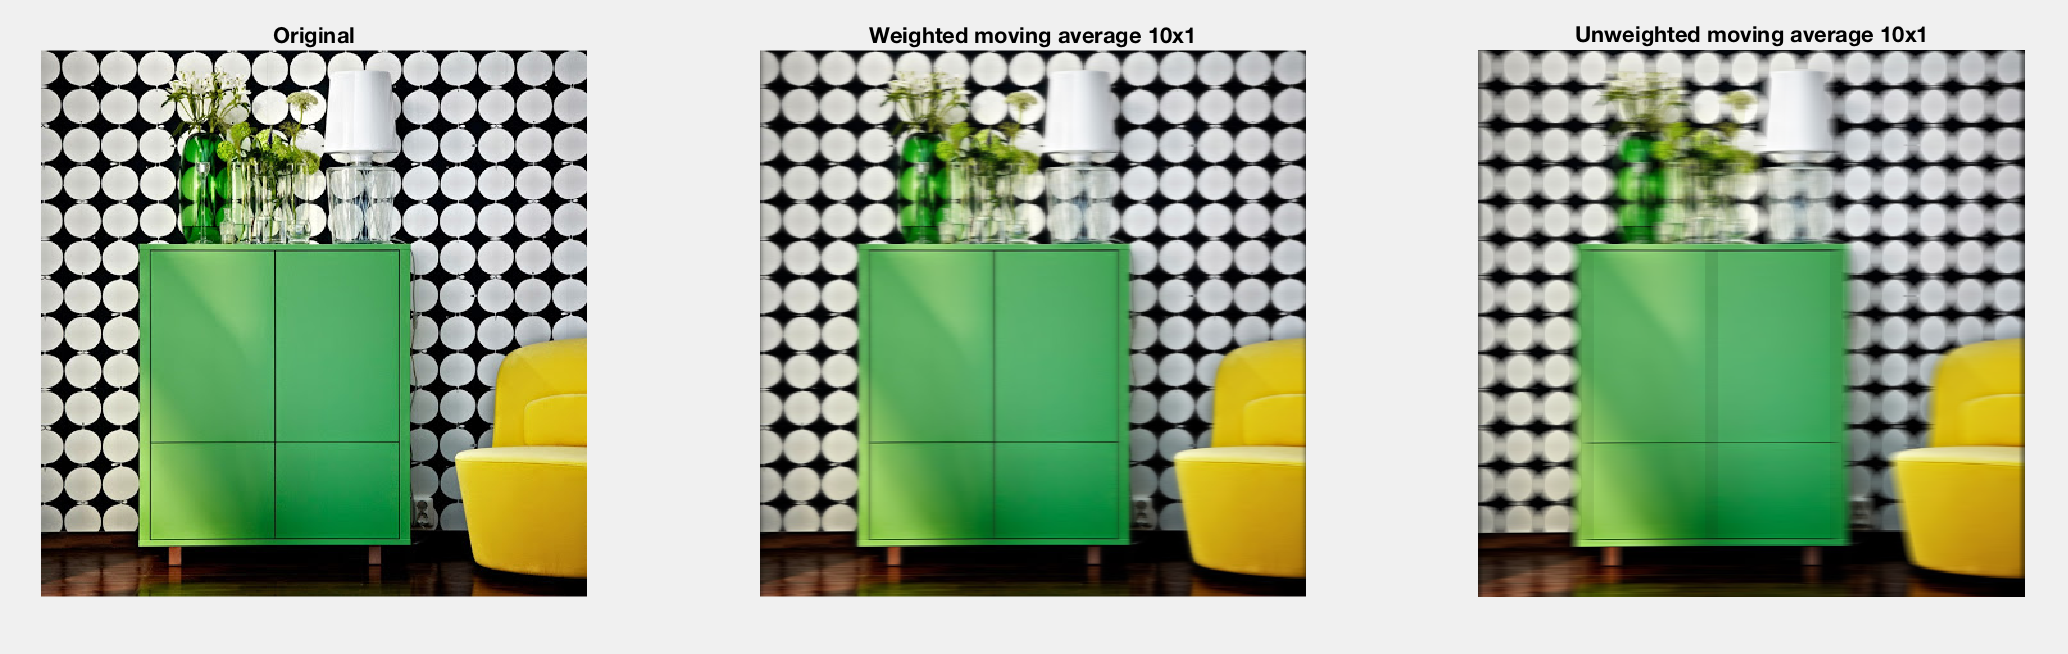
\includegraphics[width=\textwidth]{task11}
  \caption{Weighted and unweighted horizontal moving average}
  \label{fig:task11}
\end{figure}

In many cases it is a wanted effect to regard pixels in close proximity to the target pixel more highly than the ones that are further away. This can elegantly be achieved by applying a gaussian kernel, like the ones depicted in figure \ref{fig:task12}. Each gaussian kernel has to parameters: kernel size and sigma. The kernel size determines the maximum area in which pixels are considered to compute the filtered value of the target pixel. The value of sigma determines, how much stronger close neighbors are weighted, than distant neighbors. A small sigma results in close neighbors being weighted much higher than with a large sigma.

\begin{figure}[!hbt]
  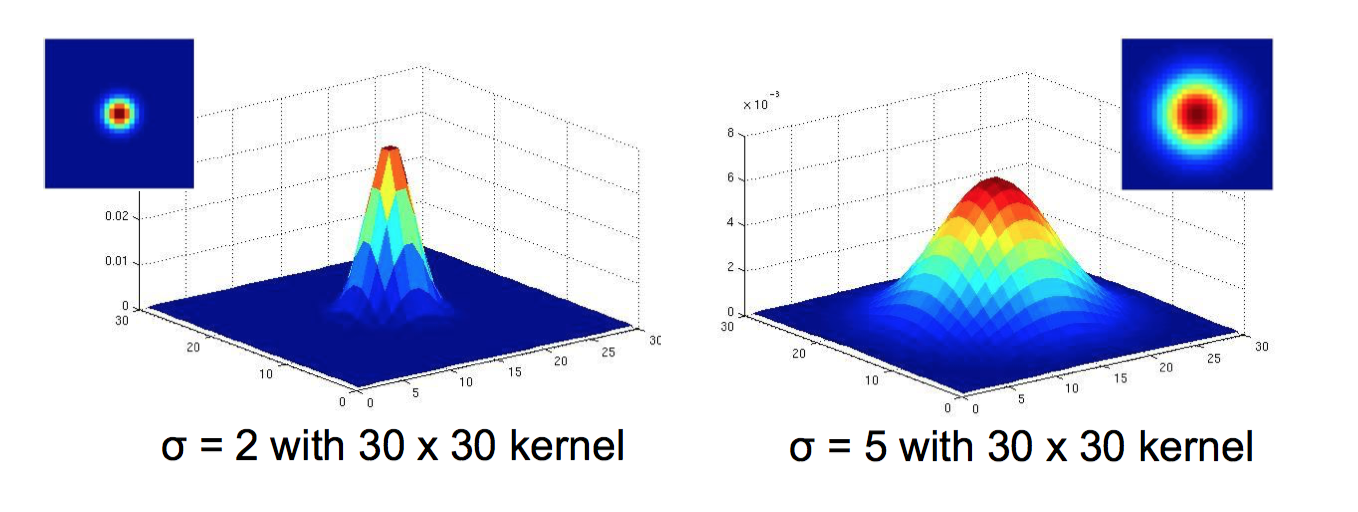
\includegraphics[width=\textwidth]{task12}
  \caption{Two differently parameterized gaussian kernels}
  \label{fig:task12}
\end{figure}

Figure \ref{fig:task13} shows the effect of different kernel sizes of a gaussian filter. The left image used a kernel with area 10x10 pixels and the right image with a kernel of 30x30 pixels is clearly more blurry with more details and noise removed.

\begin{figure}[!hbt]
  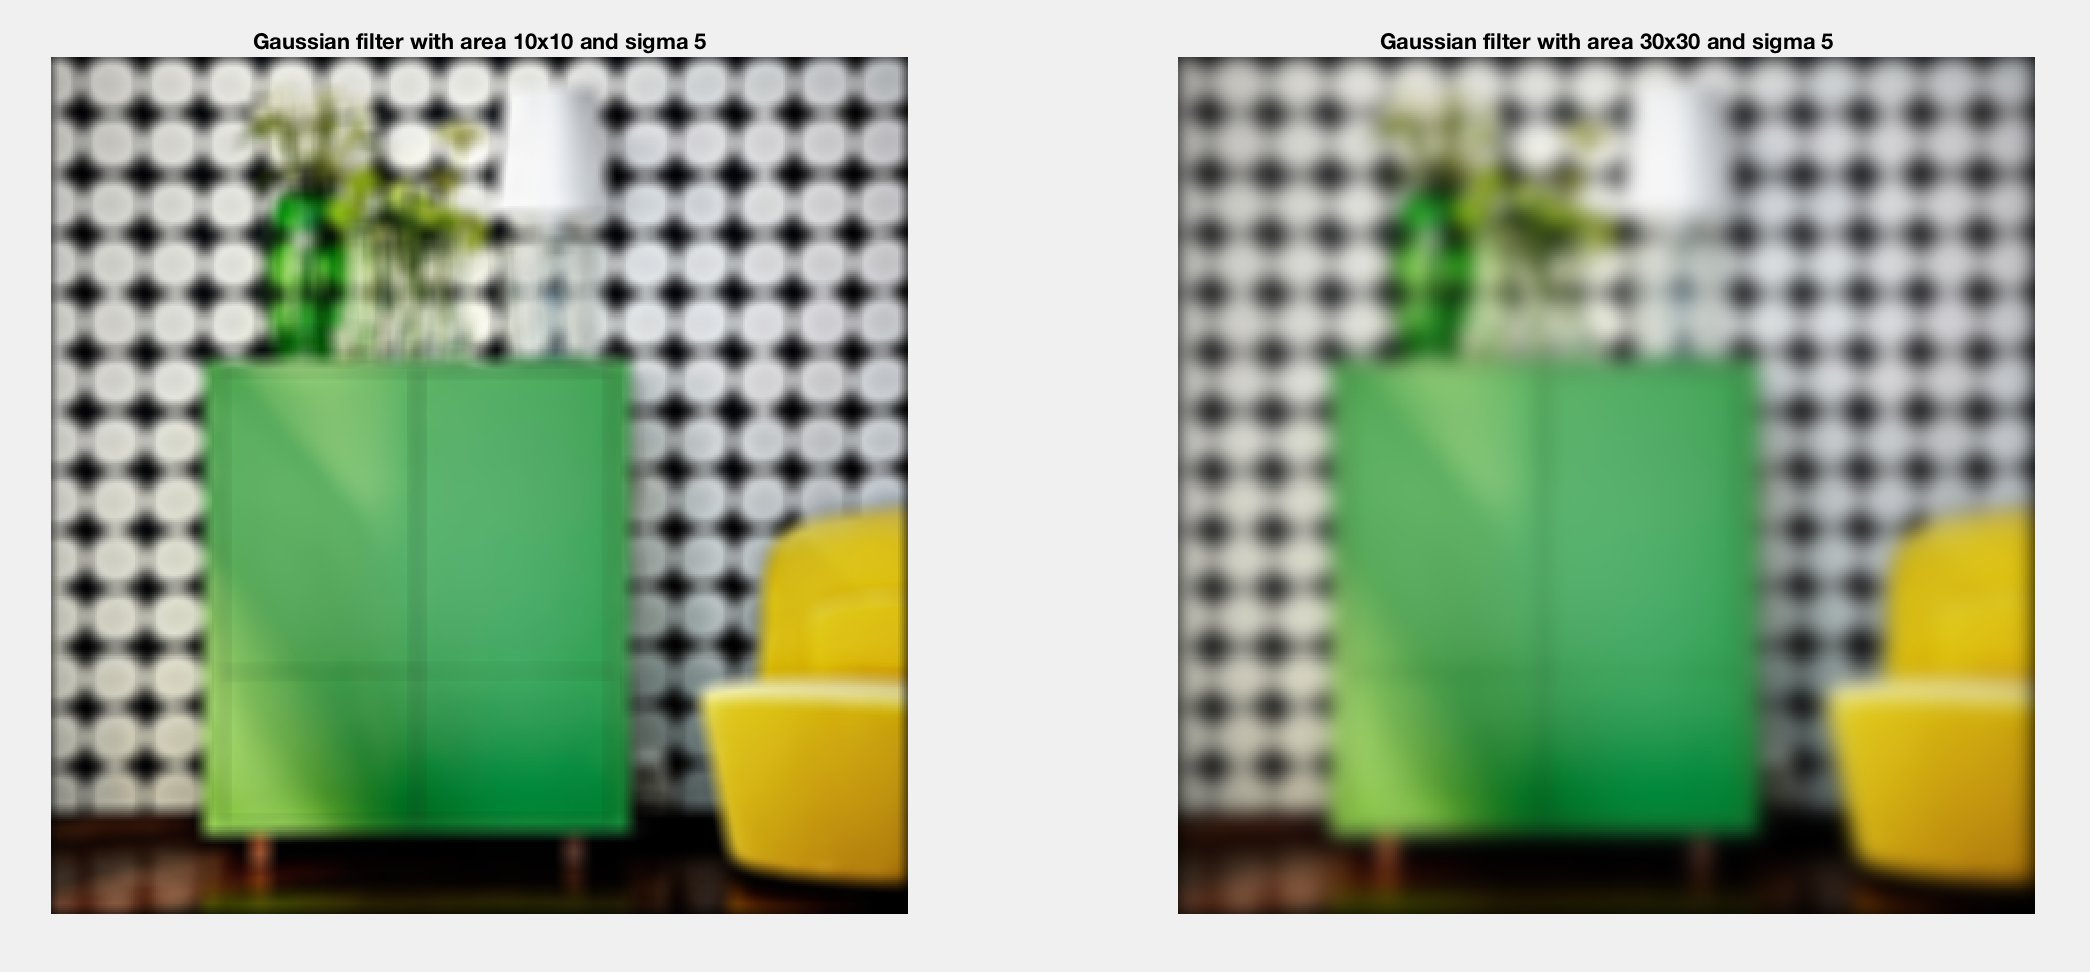
\includegraphics[width=\textwidth]{task13}
  \caption{Gaussian kernels with different areas}
  \label{fig:task13}
\end{figure}

As described before, the choice of sigma for gaussian kernels also influences their effect. This can be seen in figure \ref{fig:task14}.

\begin{figure}[!hbt]
  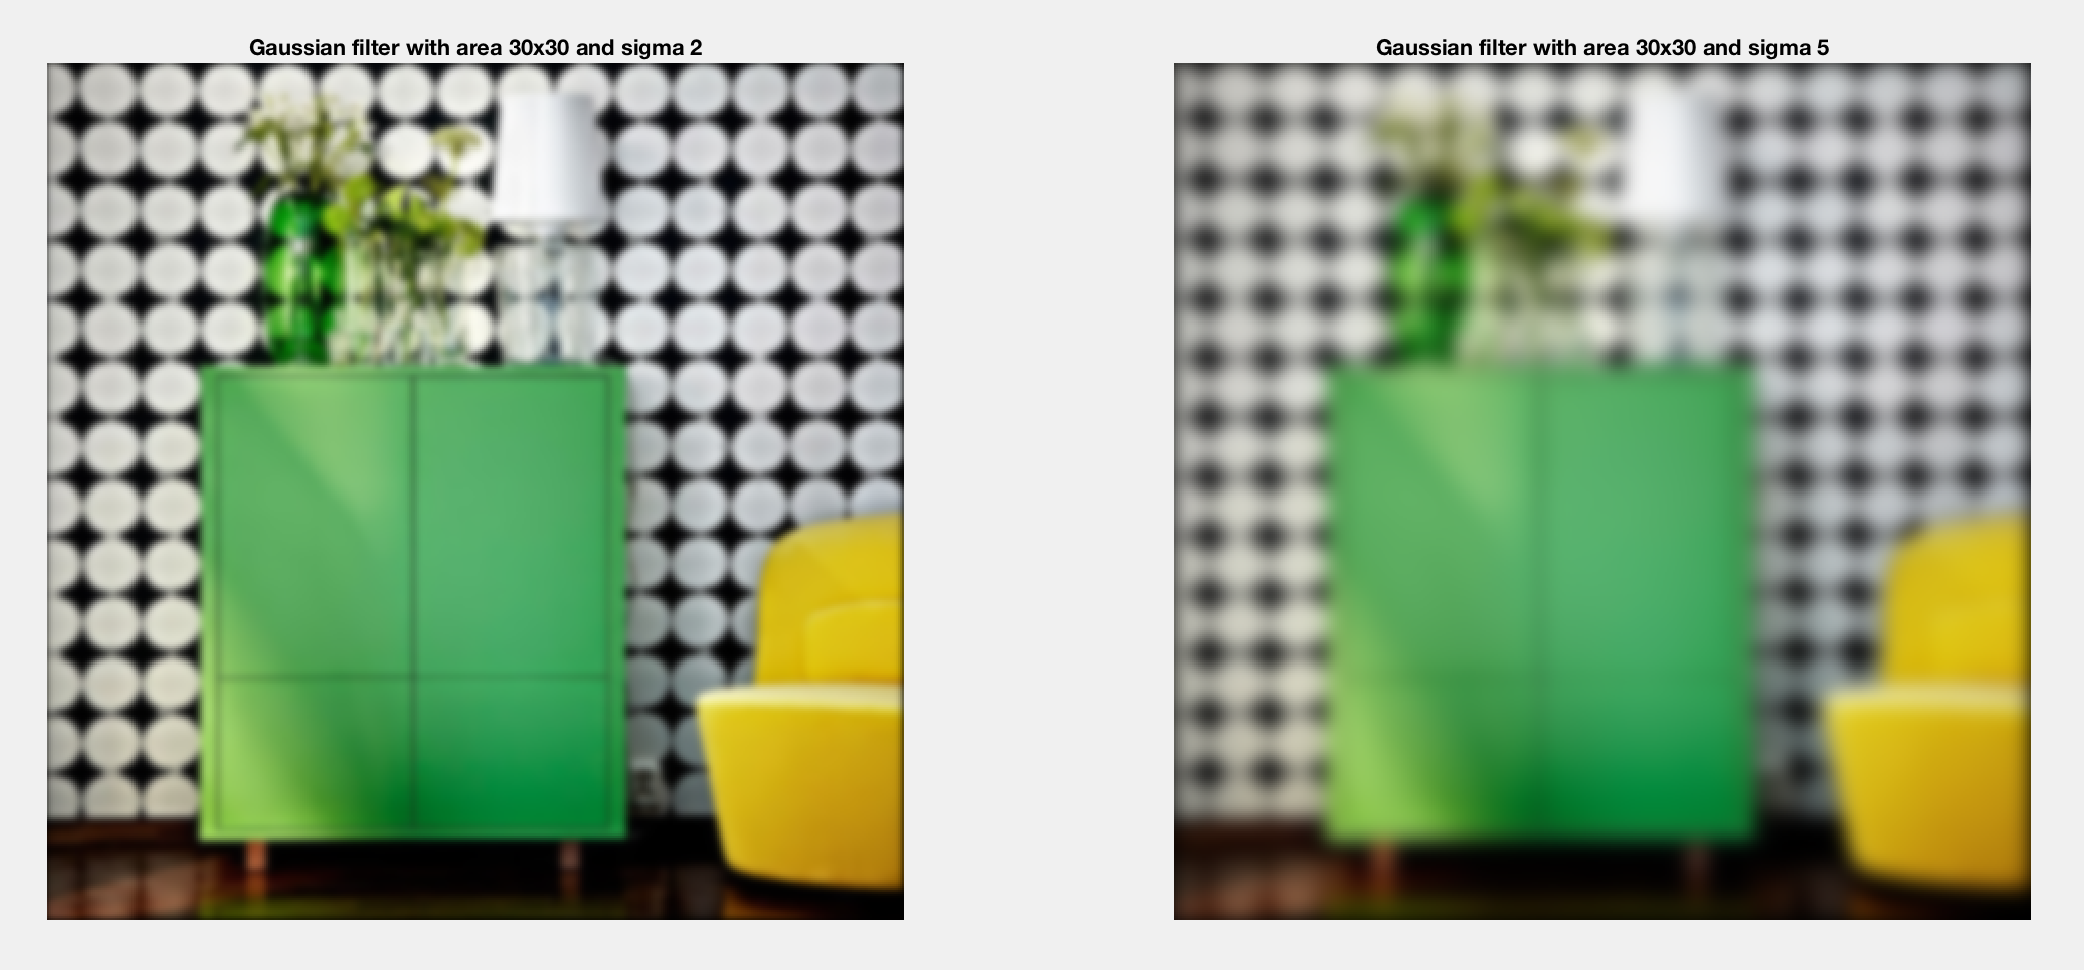
\includegraphics[width=\textwidth]{task14}
  \caption{Gaussian kernels with different sigmas}
  \label{fig:task14}
\end{figure}

The inbuilt function \textit{imfilter} in Matlab can use both custom filters like the weighted average and predefined filters like the gaussian on both RGB- and grayscale-images. Even though the kernel is 2-dimensional, the function can apply it sequentially on all three channels of the three-dimensional RGB-images.

It is important to normalize kernels in convolution filtering in order to keep values of the image generally in the same range of values like before. If normalization does not happen, the filtered image will have far higher values and eventually turn into a simple white image. This effect can be seen in figure \ref{fig:task15}.

\begin{figure}[!hbt]
  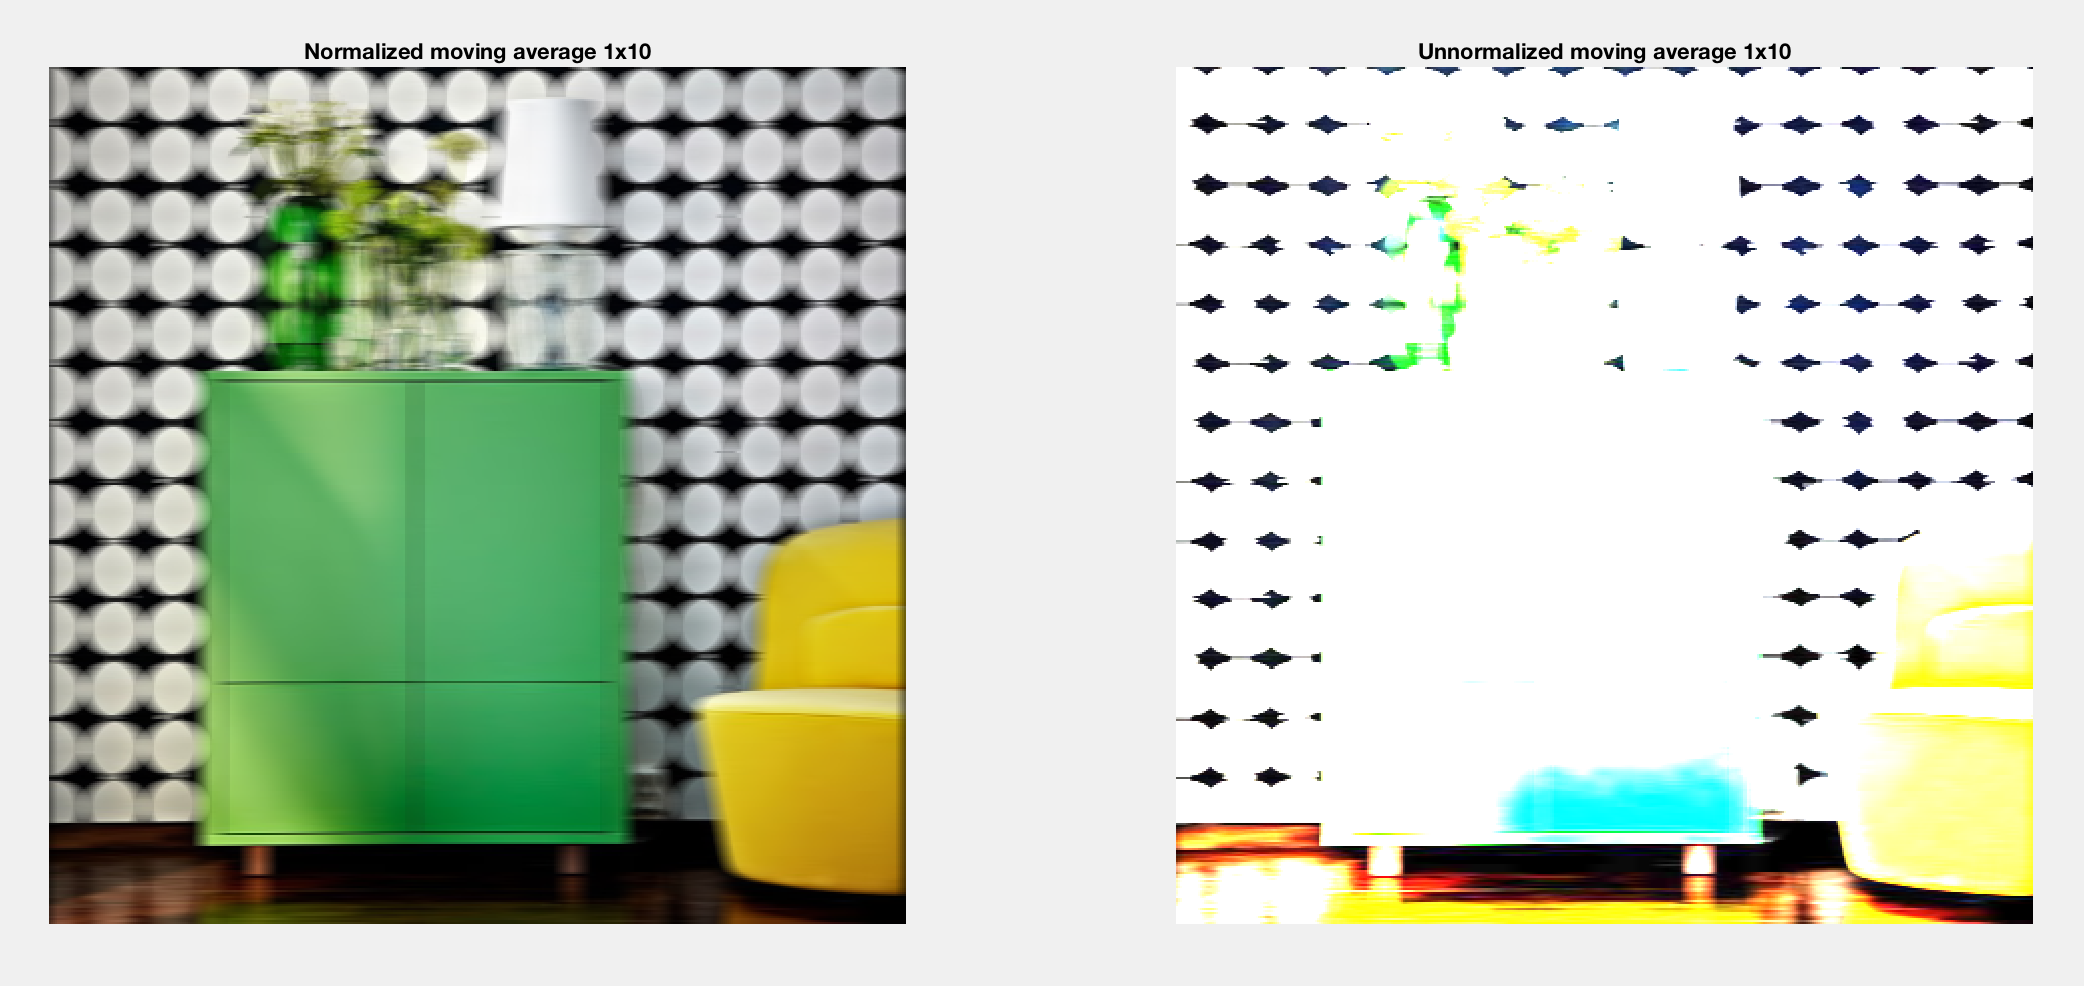
\includegraphics[width=\textwidth]{task15}
  \caption{The importance of normalizing kernels}
  \label{fig:task15}
\end{figure}

It is also possible to apply the same filter iteratively more than once to an image. The effect can be observed in figure \ref{fig:task16}

\begin{figure}[!hbt]
  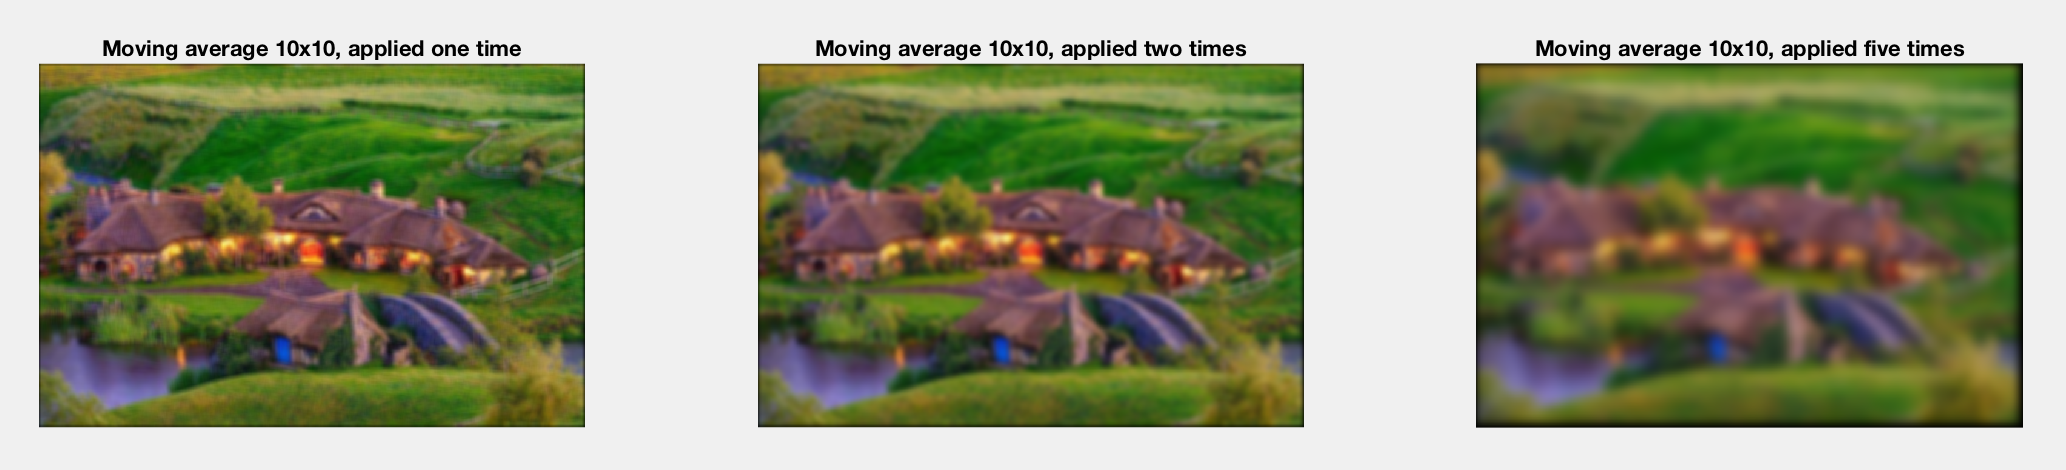
\includegraphics[width=\textwidth]{task16}
  \caption{Applying filters multiple times}
  \label{fig:task16}
\end{figure}

When calculating the absolute difference between a smoothed image and its original, an effect as in figure \ref{fig:task17}. Areas of the image that have very similar pixels stay don't change a lot when smoothing the picture and hence look black (near zero values) on the difference image. Only in areas of the image where pixels change more drastically, the difference shows higher values. This can be seen as some first step of edge detection.

\begin{figure}[!hbt]
  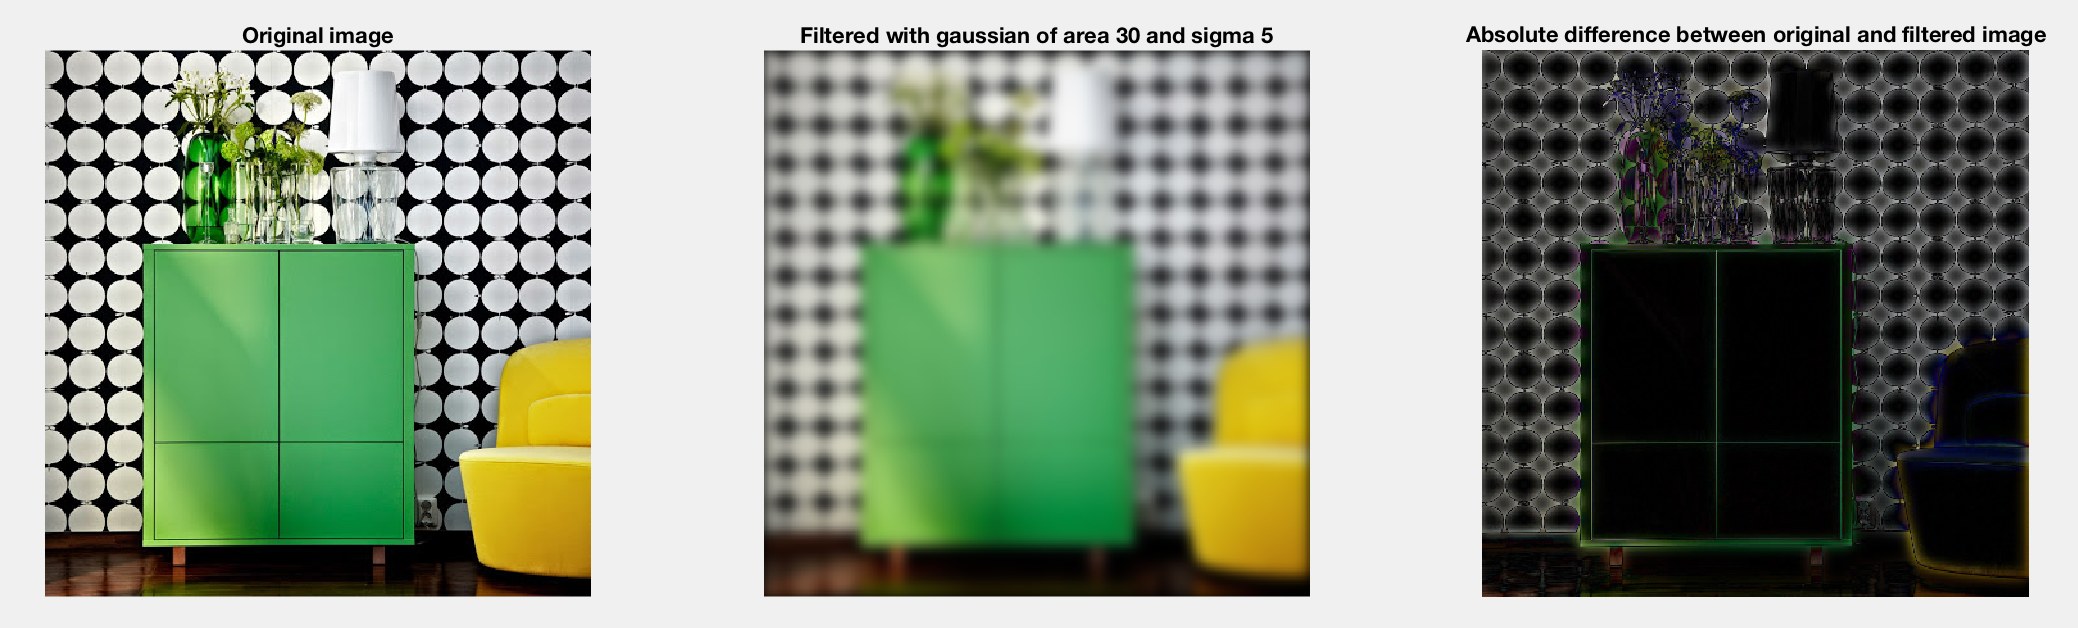
\includegraphics[width=\textwidth]{task17}
  \caption{Absolute difference between a smoothed image and its original}
  \label{fig:task17}
\end{figure}

\section*{Exercise 4:}

The wanted effect of swapping the two halves of the image can be achieved by simple concatenation with the Matlab function \textit{horzcat}. For details see the file \texttt{exercise4.m}.

\begin{figure}[!hbt]
  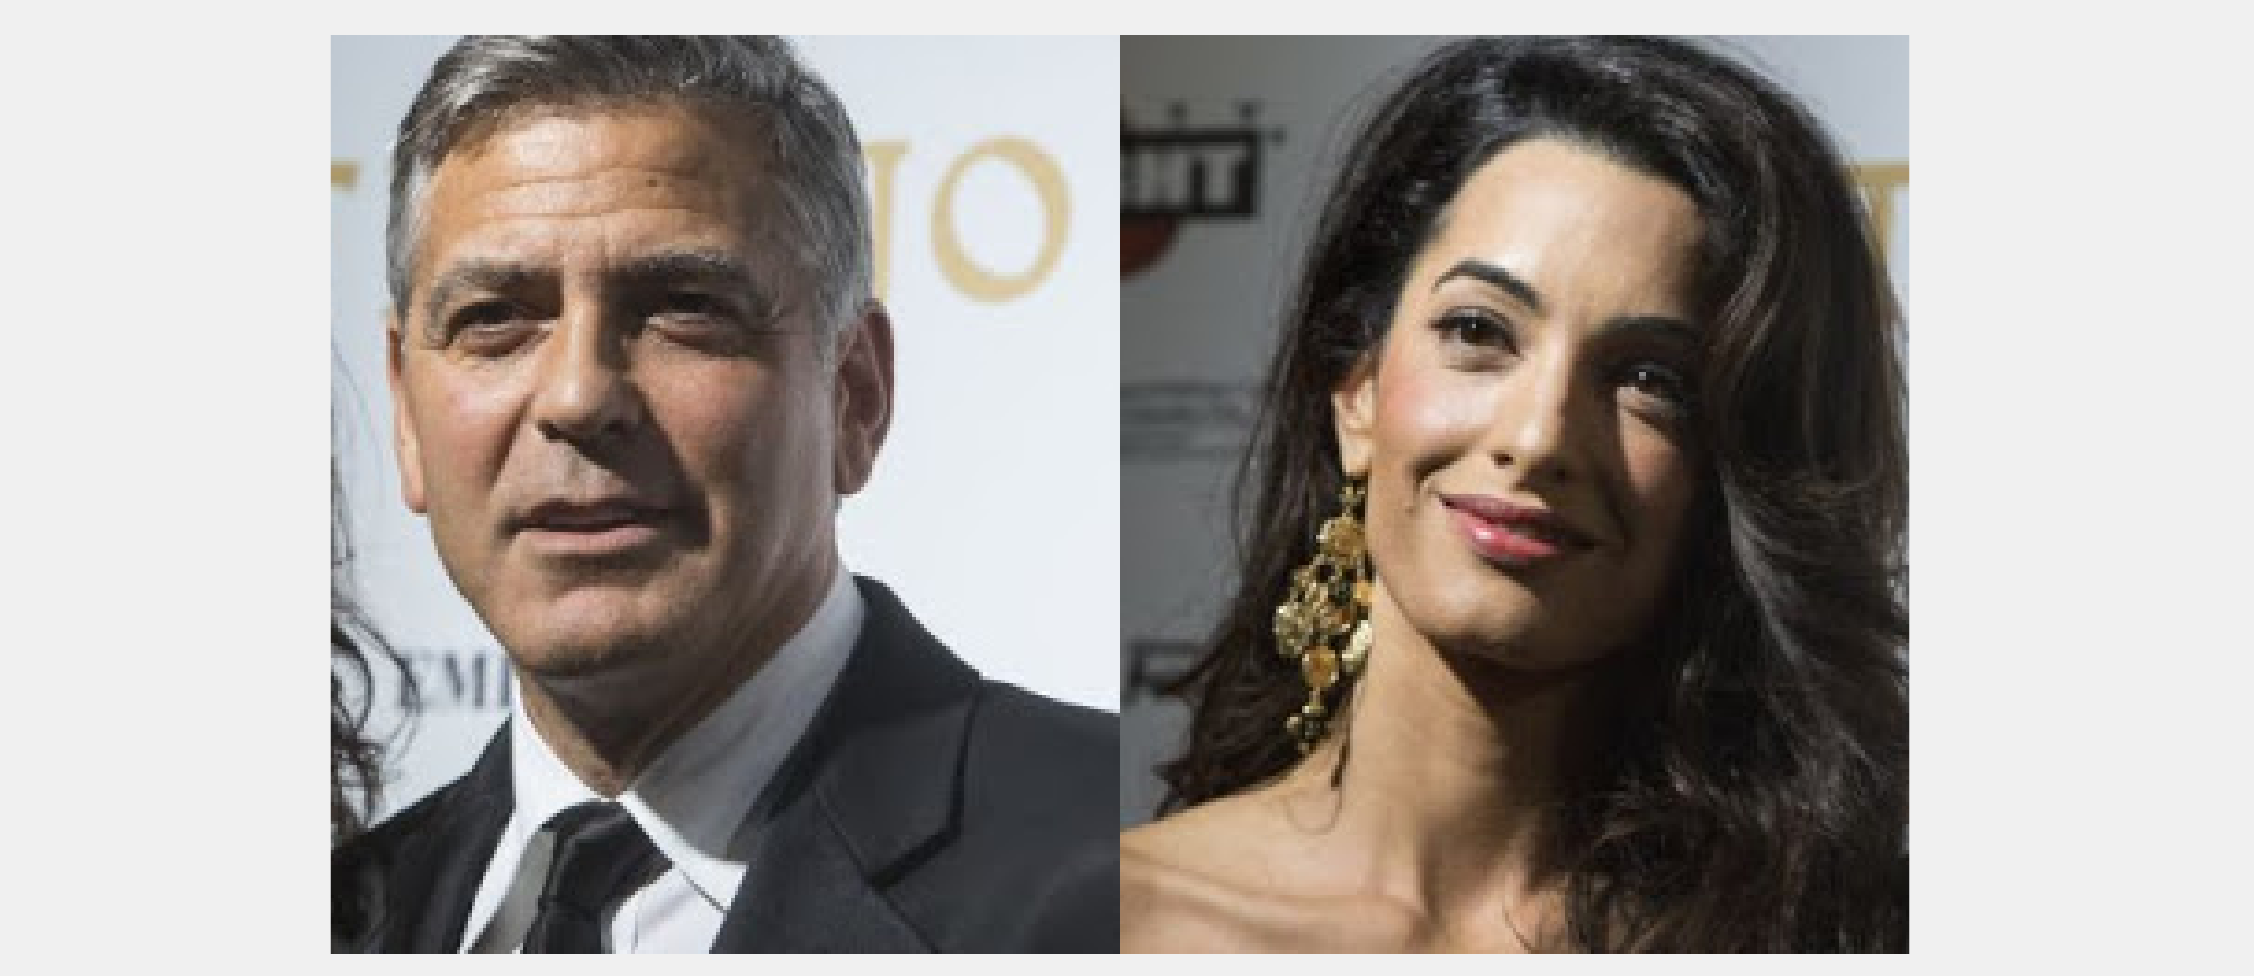
\includegraphics[width=\textwidth]{task18}
  \caption{Image halves swapped}
  \label{fig:task18}
\end{figure}

\section*{Exercise 5:}

The inbuilt Matlab function \textit{imbinarize} creates a logical array for an grayscale image I given a threshold t in which all pixels with values above t get mapped to a 1 and all other pixels to a 0.

Figure \ref{fig:task19} shows binarizations for a grayscale image of a car for different thresholds. It can be seen that it depends heavily on the specific image which threshold results in a useful binarization. In this case, a threshold of 20 or 30 still maps most pixel to white pixels and does not yield a useful result. When moving the threshold closer to 1, most pixels get mapped to a black output, as the in the last image of figure \ref{fig:task19}.

\begin{figure}[!hbt]
  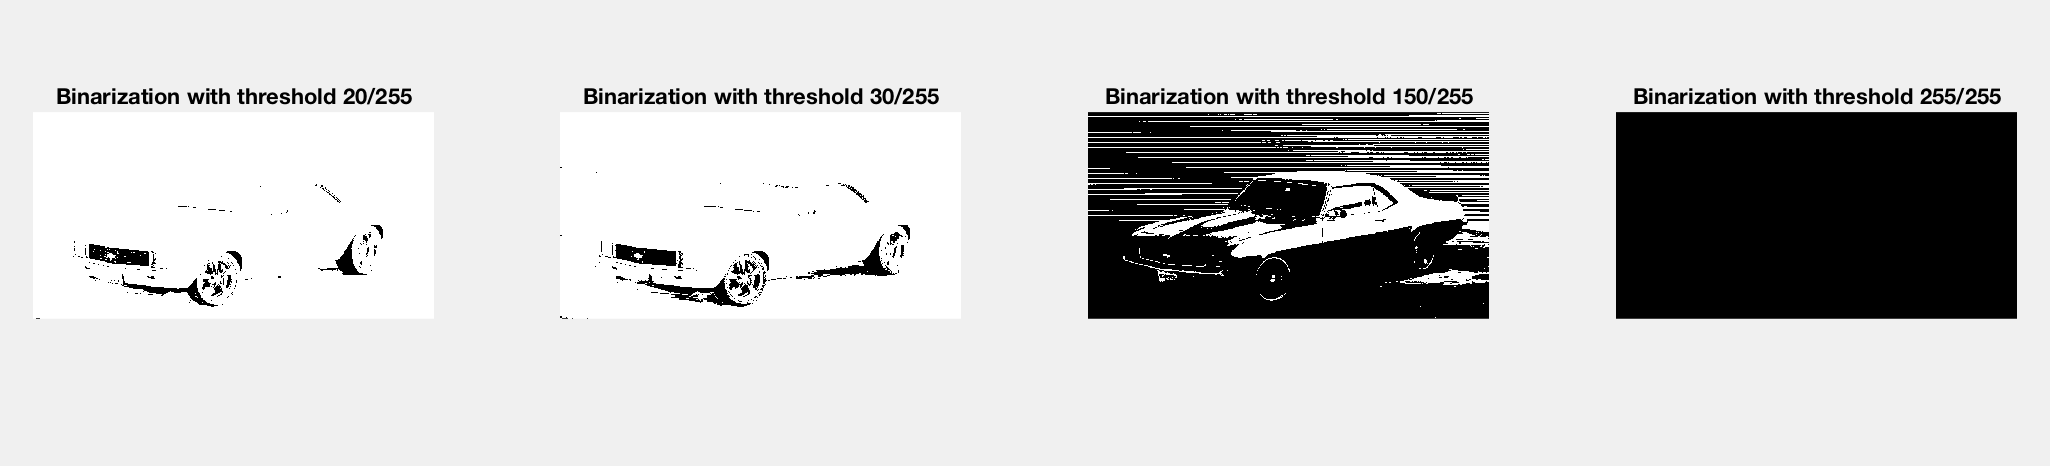
\includegraphics[width=\textwidth]{task19}
  \caption{Image binarization with different thresholds}
  \label{fig:task19}
\end{figure}

Figure \ref{fig:task20} shows the pixel-wise product of the original image and its binarization with a threshold of 150/250.

\begin{figure}[!hbt]
  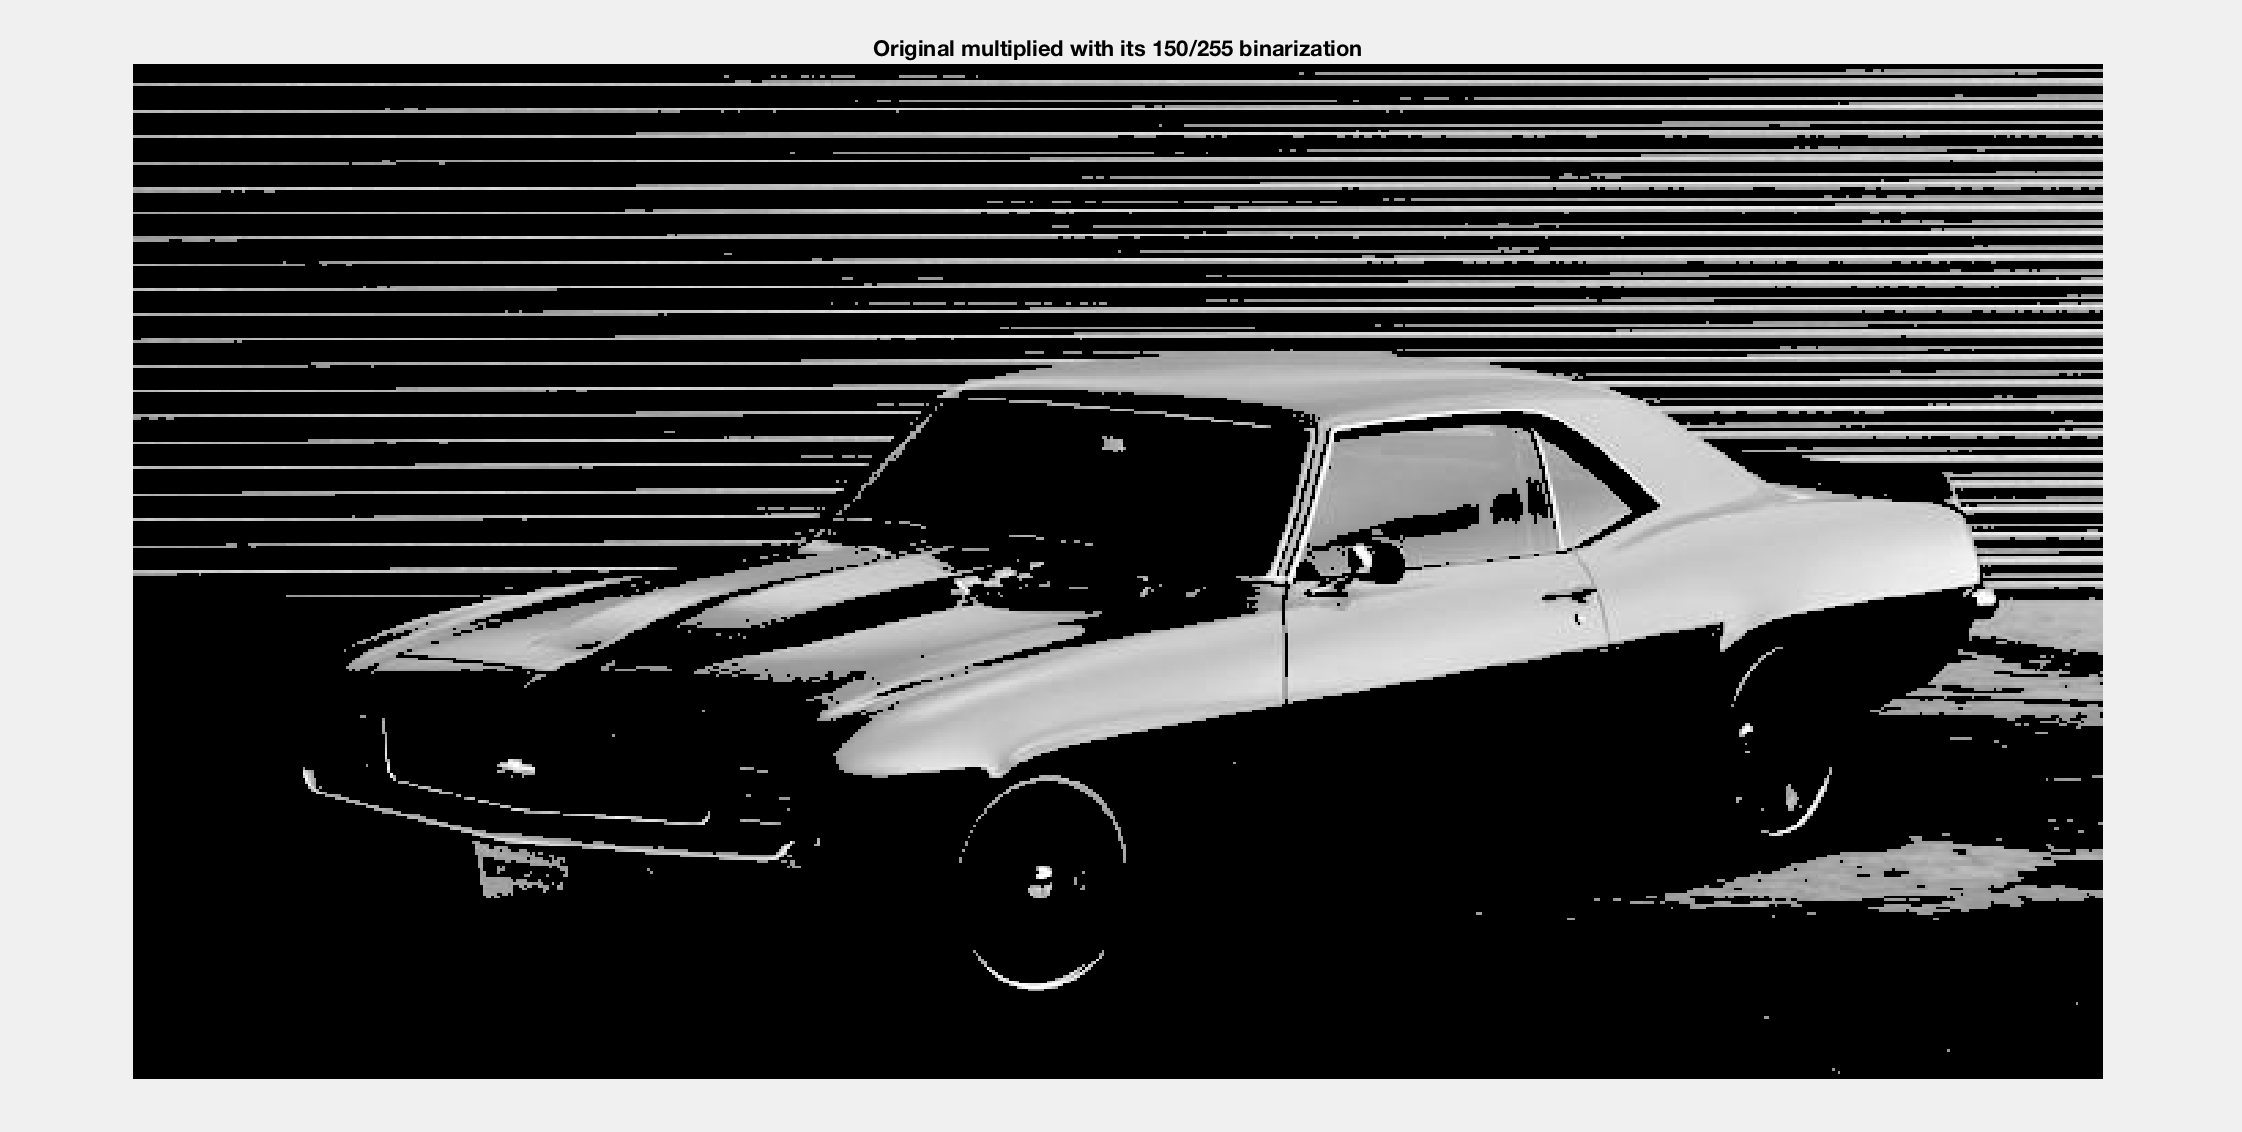
\includegraphics[width=\textwidth]{task20}
  \caption{Original multiplied with its binarization}
  \label{fig:task20}
\end{figure}

Figure \ref{fig:task21} shows the pixel-wise product of the original image and its inverted binarization with a threshold of 150/250.

\begin{figure}[!hbt]
  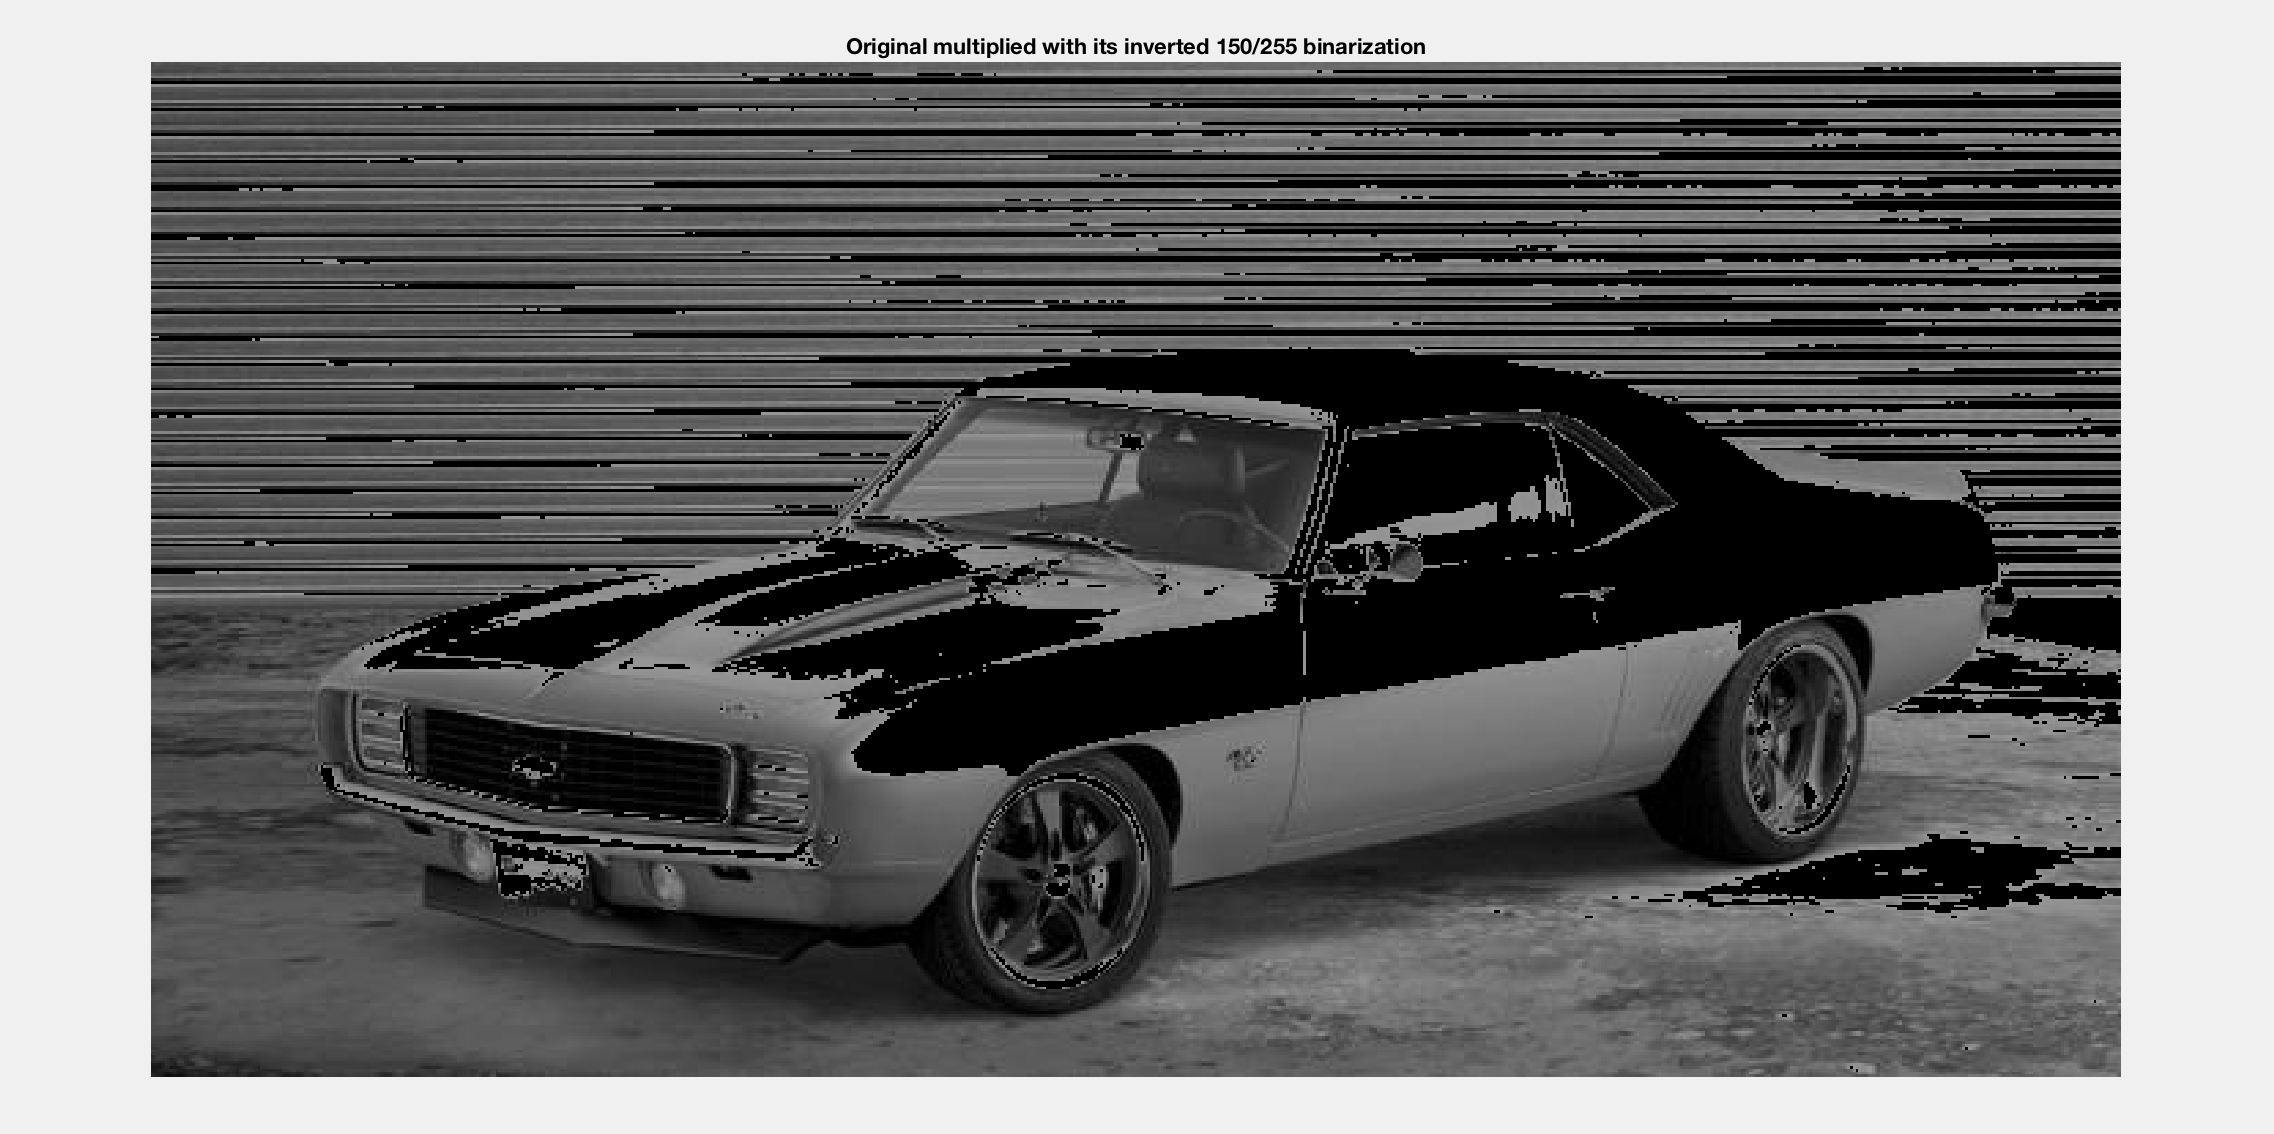
\includegraphics[width=\textwidth]{task21}
  \caption{Original multiplied with its inverted binarization}
  \label{fig:task21}
\end{figure}

\section*{Exercise 6:}

In exercise 6, the pixels showing a hand are extracted from the black background of an image and copied onto a second image. The commands used for this process can be found in \texttt{exercise6.m}. The resulting image is depicted in figure \ref{fig:task22}.

\begin{figure}[!hbt]
  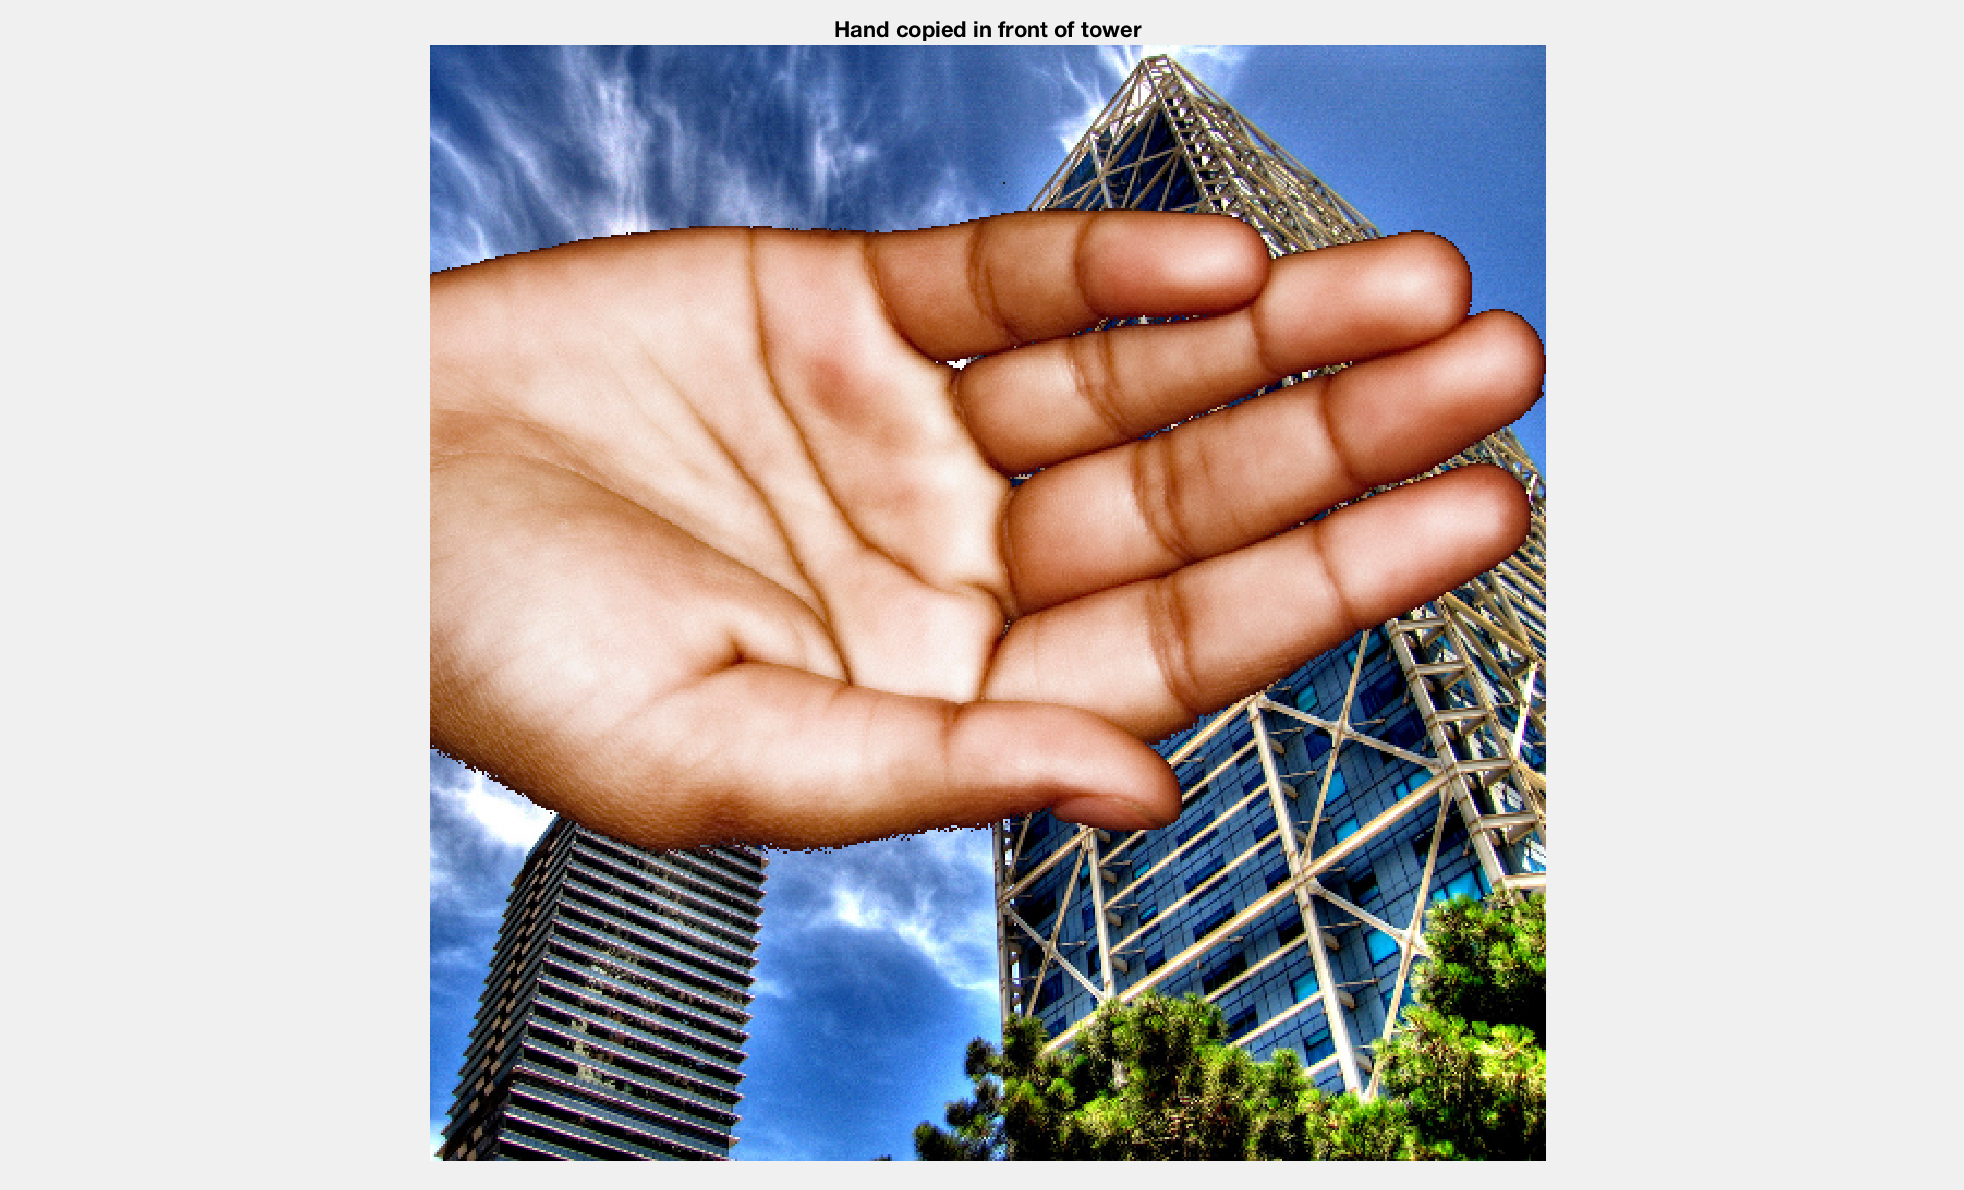
\includegraphics[width=\textwidth]{task22}
  \caption{Hand copied in front of tower}
  \label{fig:task22}
\end{figure}

\end{document}
